\documentclass[11pt,a4paper,oneside]{report}

\usepackage[utf8]{inputenc}
\usepackage[T1]{fontenc}
\usepackage[italian]{babel}
\usepackage{lmodern}
\usepackage{microtype}
\usepackage{graphicx}
\usepackage{caption}
\captionsetup{font={small,sf}, labelfont=bf}
\usepackage[top=2.5cm, bottom=2.5cm, left=2.5cm, right=2.5cm]{geometry}

\usepackage{amsmath,amssymb,amsthm,mathtools,bm}
\usepackage{booktabs}
\usepackage{tabularx}
\usepackage{array}
\usepackage{enumitem}
\usepackage{fancyhdr}
\usepackage{titlesec}
\usepackage{xcolor}
\usepackage[most]{tcolorbox}
\usepackage{tikz}
\usetikzlibrary{arrows.meta, patterns, calc, decorations.pathmorphing}

\usepackage[colorlinks=true,
            linkcolor=blue!80!black,
            citecolor=teal!80!black,
            urlcolor=cyan!80!black,
            bookmarksdepth=3]{hyperref}

% Palette cromatica perenne tema chiaro (WCAG AAA)
\definecolor{primaryBlue}{RGB}{24, 76, 120}
\definecolor{slateBg}{RGB}{248, 250, 252}
\definecolor{slateBorder}{RGB}{203, 213, 225}
\definecolor{accentGreen}{RGB}{22, 163, 74}
\definecolor{accentAmber}{RGB}{217, 119, 6}
\definecolor{accentRed}{RGB}{220, 38, 38}

% Box didattici specialistici (Zero Rubriche / Nessun punteggio)
\newtcolorbox{leggefisica}[1][]{
  enhanced, breakable, colback=slateBg, colframe=primaryBlue,
  fonttitle=\bfseries\sffamily, title={Principio e Legge Fisica: #1},
  arc=3mm, boxrule=1pt, top=3.5mm, bottom=3.5mm, left=4mm, right=4mm
}

\newtcolorbox{commento}[1][]{
  enhanced, breakable, colback=accentAmber!6!white, colframe=accentAmber,
  fonttitle=\bfseries\sffamily, title={Interpretazione Fisica e Intuizione Didattica: #1},
  arc=3mm, boxrule=0.8pt, top=3.5mm, bottom=3.5mm, left=4mm, right=4mm
}

\newtcolorbox{problema}[1][]{
  enhanced, breakable, colback=white, colframe=accentGreen,
  fonttitle=\bfseries\sffamily, title={Problema Risolto a 9 Fasi: #1},
  arc=3mm, boxrule=0.8pt, top=3.5mm, bottom=3.5mm, left=4mm, right=4mm
}

\newtcolorbox{boxlibro}[1][]{
  enhanced, breakable, colback=white, colframe=slateBorder,
  fonttitle=\bfseries\sffamily\color{primaryBlue}, title={Dal Testo Scolastico: #1},
  arc=2mm, boxrule=0.6pt, top=3mm, bottom=3mm, left=3.5mm, right=3.5mm
}

\pagestyle{fancy}
\fancyhf{}
\fancyhead[L]{\small\sffamily Liceo Scientifico Statale «Leonardo da Vinci» – Maglie}
\fancyhead[R]{\small\sffamily Fisica – Classe 4B}
\fancyfoot[C]{\thepage}
\renewcommand{\headrulewidth}{0.4pt}

\titleformat{\chapter}[display]
  {\normalfont\sffamily\huge\bfseries\color{primaryBlue}}
  {\chaptertitlename\ \thechapter}{15pt}{\Huge}

\begin{document}

% Frontespizio Ufficiale
\begin{titlepage}
\begin{center}
  \vspace*{1cm}
  {\Large\textbf{LICEO SCIENTIFICO STATALE «LEONARDO DA VINCI»}}\\[0.3cm]
  {\large\textbf{MAGLIE (LE)}}\\[2cm]
  \rule{\textwidth}{1.5pt}\\[0.5cm]
  {\Huge\textbf{\color{primaryBlue} TERMODINAMICA DEI GAS PERFETTI}}\\[0.4cm]
  {\Large\textbf{MODELLO CINETICO-MOLECOLARE, PIANO DI CLAPEYRON ED EQUAZIONE DI STATO}}\\[0.5cm]
  \rule{\textwidth}{1.5pt}\\[2.2cm]
  
  \begin{minipage}{0.45\textwidth}
    \textbf{Docente:}\\
    Prof. Giuseppe De Pascali\\
    \textit{Matematica e Fisica}
  \end{minipage}
  \hfill
  \begin{minipage}{0.45\textwidth}
    \raggedleft
    \textbf{Classe:}\\
    4ª Sezione B\\
    \textit{Liceo Scientifico Tradizionale}\\
    Anno Scolastico 2026/2027
  \end{minipage}

  \vfill
  {\small Compendio Didattico Rigoroso con Tracce Originali Ritagliate dal Testo e Commenti Fenomenologici (Standard Master 4.0)}
\end{center}
\end{titlepage}

\tableofcontents
\newpage

% ==============================================================================
% CAPITOLO 1
% ==============================================================================
\chapter{Le Leggi Sperimentali dei Gas e la Scala Kelvin}

La termodinamica descrive il comportamento della materia attraverso variabili macroscopiche di stato: pressione $p$, volume $V$ e temperatura $t$. Nello studio degli stati gassosi a bassa densità e temperature sufficientemente lontane dalla liquefazione, il comportamento reale si approssima con straordinaria precisione al modello ideale del \textbf{gas perfetto}. Storicamente, le proprietà dei gas sono state scoperte mediante tre fondamentali leggi sperimentali, ciascuna ottenuta mantenendo costante una delle tre coordinate termodinamiche.

\section{La Trasformazione Isoterma e la Legge di Boyle-Mariotte}
Nel 1662 Robert Boyle e indipendentemente Edme Mariotte (1676) stabilirono il legame tra volume e pressione a temperatura costante ($T = \text{cost}$).

\begin{leggefisica}[Legge di Boyle-Mariotte]
A temperatura costante, il volume occupato da una determinata quantità di gas è inversamente proporzionale alla pressione esercitata su di esso:
\[
p \cdot V = \text{costante} \iff p_1 V_1 = p_2 V_2
\]
\end{leggefisica}

\begin{commento}[Meccanismo Fenomenologico dell'Isoterma]
Se un gas racchiuso in un cilindro con pistone mobile viene compresso dimezzandone il volume ($V \to V/2$), le particelle molecolari dispongono della metà dello spazio per muoversi. A parità di agitazione termica (temperatura immutata), la frequenza degli urti elastici contro l'unità di superficie delle pareti raddoppia. Di conseguenza, la pressione macroscopica raddoppia ($p \to 2p$). Nel piano di Clapeyron $(V, p)$, la legge di Boyle è rappresentata da un ramo di \textbf{iperbole equilatera} avente per asintoti gli assi cartesiani.
\end{commento}

\section{La Trasformazione Isobara e la Prima Legge di Gay-Lussac}
Mantenendo costante la pressione del gas ($p = \text{cost}$), Joseph Louis Gay-Lussac (1802) dimostrò che la dilatazione termica di qualsiasi gas segue una legge lineare rispetto alla temperatura in gradi Celsius.

\begin{leggefisica}[Prima Legge di Gay-Lussac (Isobara)]
A pressione costante, il volume $V(t)$ occupato da una massa di gas a temperatura $t$ (in gradi Celsius) varia secondo la legge lineare:
\[
V(t) = V_0 \, (1 + \alpha \, t)
\]
dove $V_0$ è il volume occupato alla temperatura di $0\,{^\circ}\text{C}$ e $\alpha$ è il \textbf{coefficiente di dilatazione volumica}, universale per tutti i gas perfetti:
\[
\alpha \approx \frac{1}{273{,}15}\,{^\circ}\text{C}^{-1} \approx 3{,}661 \cdot 10^{-3}\,{^\circ}\text{C}^{-1}
\]
\end{leggefisica}

\begin{commento}[Universalità del Coefficiente $\alpha$]
A differenza dei solidi e dei liquidi, i cui coefficienti di dilatazione dipendono fortemente dalla struttura chimica del materiale, tutti i gas rarefatti condividono esattamente lo stesso valore di $\alpha$. Questo accade perché le forze attrattive intermolecolari nei gas sono del tutto trascurabili rispetto all'energia cinetica di agitazione termica, rendendo il comportamento termico puramente geometrico.
\end{commento}

\section{La Trasformazione Isocora e la Seconda Legge di Gay-Lussac}
Se il gas è confinato in un contenitore rigido indeformabile, il suo volume non può variare ($V = \text{cost}$). In questo caso, l'incremento di temperatura produce un aumento lineare della pressione.

\begin{leggefisica}[Seconda Legge di Gay-Lussac (Isocora)]
A volume costante, la pressione $p(t)$ esercitata da un gas a temperatura $t$ in Celsius varia secondo la relazione:
\[
p(t) = p_0 \, (1 + \alpha \, t)
\]
dove $p_0$ è la pressione misurata a $0\,{^\circ}\text{C}$ e $\alpha \approx \frac{1}{273{,}15}\,{^\circ}\text{C}^{-1}$ è il medesimo coefficiente di dilatazione termica.
\end{leggefisica}

\section{L'Estrapolazione allo Zero Assoluto e la Scala Kelvin}
Le formulazioni di Gay-Lussac contengono un'implicazione concettuale di straordinaria portata fisica: se estrapoliamo la retta del volume o della pressione verso temperature negative, esiste una temperatura alla quale la pressione (o il volume teorico) si annullerebbe.

Ponendo $p(t) = 0$:
\[
p_0 (1 + \alpha t) = 0 \implies 1 + \alpha t = 0 \implies t = -\frac{1}{\alpha} = -273{,}15\,{^\circ}\text{C}
\]

\begin{figure}[htbp]
\centering
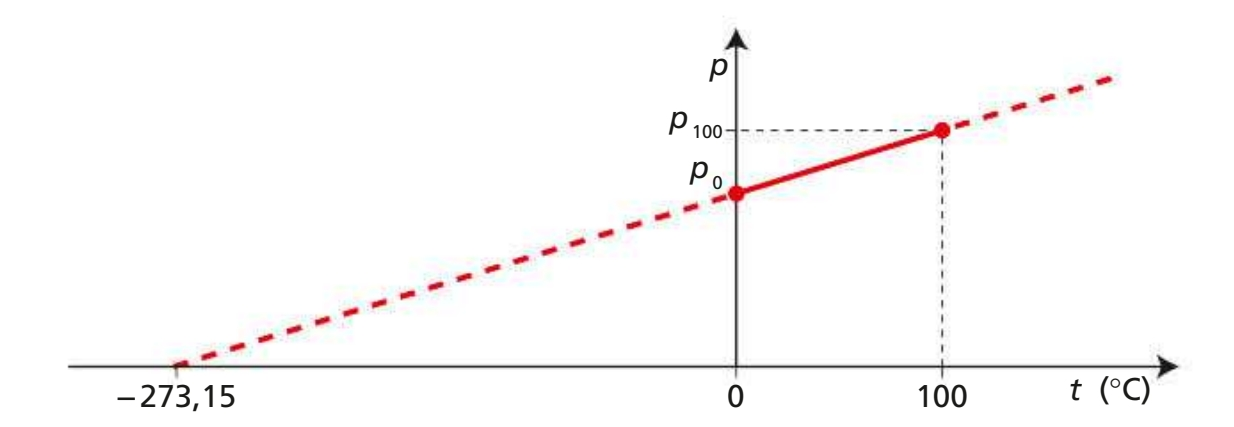
\includegraphics[width=0.78\linewidth]{immagini/grafico_zero_assoluto.jpg}
\caption{Ritaglio dal testo scolastico: estrapolazione lineare della pressione e del volume allo Zero Assoluto ($-273{,}15\,{^\circ}\text{C}$).}
\label{fig:zero_assoluto_testo}
\end{figure}

\begin{figure}[htbp]
\centering
\begin{tikzpicture}[scale=0.95]
  % Griglia tenue
  \draw[step=1cm, slateBorder!40, very thin] (-6.5,-0.5) grid (5.5,4.5);
  
  % Asse temperature
  \draw[->, thick, primaryBlue] (-6.5,0) -- (5.5,0) node[below right, font=\small\sffamily] {$t \, [{^\circ}\text{C}]$};
  % Asse pressione / volume
  \draw[->, thick, primaryBlue] (0,-0.5) -- (0,4.5) node[above left, font=\small\sffamily] {$p \text{ oppure } V$};

  % Tacca 0 C
  \draw[thick] (0,0.1) -- (0,-0.1) node[below, font=\footnotesize] {$0$};
  % Tacca 100 C
  \draw[thick] (2.5,0.1) -- (2.5,-0.1) node[below, font=\footnotesize] {$100$};
  % Tacca -273.15 C
  \draw[thick, accentRed] (-5.463,0.1) -- (-5.463,-0.1) node[below, font=\footnotesize\bfseries, fill=white, inner sep=1pt] {$-273{,}15$};

  % Retta sperimentale solida (t >= 0)
  \draw[very thick, primaryBlue] (0, 1.8) -- (4.5, 3.28) node[right, font=\small\bfseries] {Gas misurato ($t \ge 0\,{^\circ}\text{C}$)};

  % Estrapolazione tratteggiata verso zero assoluto
  \draw[thick, dashed, accentRed] (0, 1.8) -- (-5.463, 0);

  % Punti notevoli
  \fill[accentAmber] (0, 1.8) circle (2.5pt) node[above left, font=\footnotesize, fill=white, inner sep=1pt] {$p_0 \text{ (a } 0\,{^\circ}\text{C)}$};
  \fill[accentRed] (-5.463, 0) circle (3pt) node[above left, font=\footnotesize\bfseries, fill=white, inner sep=1.5pt] {Zero Assoluto ($0\text{ K}$)};

  % Evidenziazione intervallo
  \node[font=\footnotesize\sffamily, accentRed, align=center] at (-3, 2.5) {Estrapolazione teorica\\$p \to 0$ per $t \to -273{,}15\,{^\circ}\text{C}$};
\end{tikzpicture}
\caption{Grafico cartesiano analitico dell'estrapolazione lineare: determinazione geometrica dello Zero Assoluto.}
\label{fig:zero_assoluto_analitico}
\end{figure}

Questa temperatura limite invalicabile costituisce lo \textbf{Zero Assoluto} della natura. Lord Kelvin (William Thomson, 1848) definì la \textbf{scala assoluta di temperatura} ponendo lo zero in corrispondenza di tale limite:
\[
\mathbf{T \, [\text{K}] = t \, [{^\circ}\text{C}] + 273{,}15}
\]

Riscrivendo le leggi di Gay-Lussac mediante la temperatura assoluta $T$ si ottiene la loro formulazione universale:
\begin{align*}
V(T) &= V_0 \left(1 + \frac{t}{273{,}15}\right) = V_0 \, \frac{273{,}15 + t}{273{,}15} = \mathbf{V_0 \, \frac{T}{T_0} \iff \frac{V_1}{T_1} = \frac{V_2}{T_2}} \quad (p = \text{cost}) \\[2mm]
p(T) &= p_0 \left(1 + \frac{t}{273{,}15}\right) = p_0 \, \frac{273{,}15 + t}{273{,}15} = \mathbf{p_0 \, \frac{T}{T_0} \iff \frac{p_1}{T_1} = \frac{p_2}{T_2}} \quad (V = \text{cost})
\end{align*}

% ==============================================================================
% CAPITOLO 2
% ==============================================================================
\chapter{L'Equazione di Stato dei Gas Perfetti e il Piano di Clapeyron}

\section{Massa Atomica, Mole e Numero di Avogadro}
Per connettere la fisica microscopica con le grandezze chimico-fisiche macroscopiche misurabili in laboratorio, si introduce la quantità di sostanza, misurata in \textbf{moli} ($\text{mol}$).
\begin{itemize}
  \item Una \textbf{mole} è la quantità di sostanza che contiene esattamente $N_A = 6{,}02214076 \cdot 10^{23}$ entità elementari (atomi o molecole). Tale costante è il \textbf{Numero di Avogadro}.
  \item L'\textbf{unità di massa atomica unificata} ($\text{u}$ o Dalton, $\text{Da}$) è pari a un dodicesimo della massa del carbonio-12: $1\,\text{u} \approx 1{,}66054 \cdot 10^{-27}\,\text{kg}$.
  \item La \textbf{massa molare} $M$ è la massa di una mole di sostanza, espressa in $\text{g/mol}$ o in $\text{kg/mol}$. Il numero di moli $n$ contenute in una massa $m$ di gas è dato da:
  \[
  n = \frac{m}{M} \qquad \text{e il numero totale di molecole è} \qquad N = n \cdot N_A
  \]
\end{itemize}

\begin{figure}[htbp]
\centering
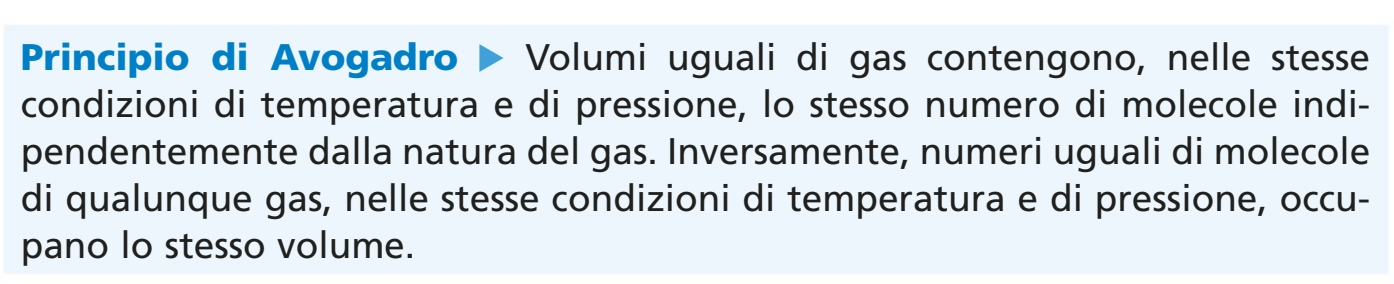
\includegraphics[width=0.88\linewidth]{immagini/box_avogadro.jpg}
\caption{Riquadro didattico dal testo scolastico: il Principio di Avogadro.}
\label{fig:avogadro_box}
\end{figure}

\begin{figure}[htbp]
\centering
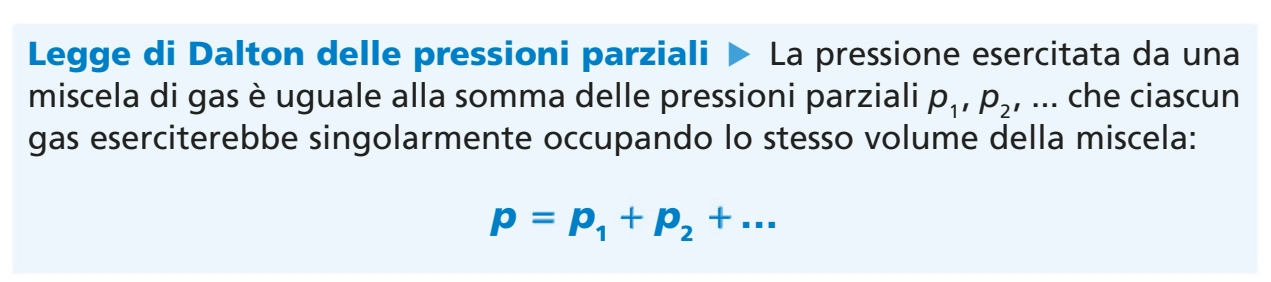
\includegraphics[width=0.88\linewidth]{immagini/box_dalton.jpg}
\caption{Riquadro didattico dal testo scolastico: la Legge di Dalton delle pressioni parziali.}
\label{fig:dalton_box}
\end{figure}

\section{L'Equazione di Stato dei Gas Perfetti (Legge di Clapeyron)}
Combinando le tre leggi empiriche (Boyle, Gay-Lussac I e Gay-Lussac II) e l'ipotesi di Avogadro in un'unica sintesi algebrica, si giunge all'equazione universale formulata da Émile Clapeyron nel 1834.

\begin{leggefisica}[Equazione di Stato di Clapeyron]
Per qualsiasi campione di gas ideale contenente $n$ moli a temperatura assoluta $T$, confinato in un volume $V$ a pressione $p$, sussiste l'identità:
\[
\mathbf{p \cdot V = n \cdot R \cdot T}
\]
dove:
\begin{itemize}
  \item $p$ è la pressione assoluta in Pascal ($\text{Pa} = \text{N/m}^2$);
  \item $V$ è il volume occupato in metri cubi ($\text{m}^3$);
  \item $n$ è il numero di moli ($\text{mol}$);
  \item $R \approx 8{,}31446\,\dfrac{\text{J}}{\text{mol}\cdot\text{K}}$ è la \textbf{Costante Universale dei Gas};
  \item $T$ è la temperatura assoluta in Kelvin ($\text{K}$).
\end{itemize}
Introducendo la \textbf{Costante di Boltzmann} $k_B = \dfrac{R}{N_A} \approx 1{,}38065 \cdot 10^{-23}\,\dfrac{\text{J}}{\text{K}}$, l'equazione di stato può essere riscritta a livello molecolare per $N$ particelle:
\[
\mathbf{p \cdot V = N \cdot k_B \cdot T}
\]
\end{leggefisica}

\begin{commento}[Condizioni Normali e Densità del Gas]
Nelle cosiddette \textbf{Condizioni Normali} (STP: $T_0 = 273{,}15\,\text{K}$, $p_0 = 1{,}01325 \cdot 10^5\,\text{Pa} = 1\,\text{atm}$), una mole di qualsiasi gas perfetto occupa il volume molare standard:
\[
V_{\text{molare}} = \frac{1\,\text{mol} \cdot R \cdot T_0}{p_0} \approx 0{,}022414\,\text{m}^3 \approx \mathbf{22{,}4\,\text{L/mol}}
\]
Esprimendo il numero di moli come $n = m/M$, l'equazione di Clapeyron lega direttamente la pressione alla densità di massa $\rho = m/V$:
\[
p \cdot V = \frac{m}{M} \, R T \implies \mathbf{p = \frac{\rho \cdot R \cdot T}{M}}
\]
Questa espressione permette di determinare sperimentalmente la massa molare o la pressione conoscendo la densità del fluido.
\end{commento}

\section{Il Piano Termodinamico di Clapeyron}
Il diagramma $(V, p)$ costituisce la rappresentazione geometrica fondamentale per visualizzare le trasformazioni di stato di un sistema fluido:

\begin{figure}[htbp]
\centering
\begin{tikzpicture}[scale=1.0]
  \draw[->, thick, primaryBlue] (0,0) -- (6.8,0) node[below right, font=\small\sffamily] {$V \, [\text{m}^3]$};
  \draw[->, thick, primaryBlue] (0,0) -- (0,5.2) node[above left, font=\small\sffamily] {$p \, [\text{Pa}]$};

  % Famiglia di isoterme (rami di iperbole equilatera p*V = cost)
  \draw[thick, primaryBlue!50, domain=0.8:6.4, samples=100] plot (\x, {2.2/\x}) node[right, font=\footnotesize] {Isoterma $T_1$};
  \draw[thick, primaryBlue!80, domain=1.0:6.4, samples=100] plot (\x, {4.2/\x}) node[right, font=\footnotesize] {Isoterma $T_2 > T_1$};
  \draw[very thick, primaryBlue, domain=1.4:6.4, samples=100] plot (\x, {6.8/\x}) node[right, font=\footnotesize\bfseries] {Isoterma $T_3 > T_2$ ($p \cdot V = nRT$)};

  % Isobara orizzontale
  \draw[very thick, accentAmber] (1.5, 3.2) -- (5.2, 3.2) node[right, font=\footnotesize\bfseries] {Isobara ($p = \text{cost}$)};

  % Isocora verticale
  \draw[very thick, accentGreen] (3.2, 0.6) -- (3.2, 4.6) node[above, font=\footnotesize\bfseries] {Isocora ($V = \text{cost}$)};

  % Asintoti cartesiani
  \node[above, gray!70, font=\scriptsize] at (0.3, 4.8) {Asintoto $V = 0$};
  \node[right, gray!70, font=\scriptsize] at (5.8, 0.2) {Asintoto $p = 0$};

  % Punti notevoli
  \fill[accentRed] (3.2, 3.2) circle (2.5pt) node[above right, font=\footnotesize, fill=white, inner sep=1pt] {$P_0$};
\end{tikzpicture}
\caption{Diagramma di Clapeyron $(V, p)$: le trasformazioni isoterme reversibili sono rappresentate da una famiglia di rami di iperbole equilatera ($p \cdot V = n R T = \text{cost}$) riferiti agli asintoti cartesiani ($V=0$ e $p=0$). All'aumentare della temperatura ($T_1 < T_2 < T_3$), i rami iperbolici si allontanano progressivamente dall'origine. Sono illustrate anche l'isobara ($p=\text{cost}$) e l'isocora ($V=\text{cost}$).}
\label{fig:clapeyron_famiglia}
\end{figure}

% ==============================================================================
% CAPITOLO 3
% ==============================================================================
\chapter{La Teoria Cinetico-Molecolare dei Gas}

\section{I Postulati della Teoria Cinetica}
La teoria cinetica, formulata da Bernoulli, Clausius, Maxwell e Boltzmann, spiega l'origine microscopica delle grandezze termodinamiche considerando il gas come un insieme di particelle in moto perpetuo e disordinato. I postulati fondamentali sono:
\begin{enumerate}
  \item \textbf{Particelle puntiformi:} il volume occupato dalle molecole è trascurabile rispetto al volume del recipiente ($V_{\text{proprio}} \ll V$);
  \item \textbf{Assenza di forze a lungo raggio:} non sussistono forze attrattive o repulsive a distanza tra le molecole (l'energia potenziale è nulla: $E_{\text{pot}} = 0$);
  \item \textbf{Moto caotico e isotropo:} le particelle si muovono continuamente a velocità casuali in tutte le direzioni dello spazio con uguale probabilità (moto browniano);
  \item \textbf{Urti perfettamente elastici:} le collisioni reciproche e contro le pareti conservano integralmente la quantità di moto e l'energia cinetica del sistema ($\Delta K = 0$).
\end{enumerate}

\section{Dimostrazione Microscopica della Pressione dei Gas}
Consideriamo una scatola cubica di spigolo $L$ e volume $V = L^3$, contenente $N$ molecole identiche di massa $m$.
Esaminiamo una singola molecola che viaggia con componente di velocità $v_x$ diretta verso una parete piana perpendicolare all'asse $x$.

\begin{figure}[htbp]
\centering
\begin{tikzpicture}[scale=0.95]
  % Scatola cubica prospettica
  \draw[thick, slateBorder] (0,0) rectangle (4,4);
  \draw[thick, slateBorder] (4,0) -- (5.5,1.5) -- (5.5,5.5) -- (4,4);
  \draw[thick, slateBorder] (0,4) -- (1.5,5.5) -- (5.5,5.5);
  \draw[dashed, slateBorder!60] (0,0) -- (1.5,1.5) -- (5.5,1.5);
  \draw[dashed, slateBorder!60] (1.5,1.5) -- (1.5,5.5);

  % Parete evidenziata
  \fill[primaryBlue!10] (4,0) -- (5.5,1.5) -- (5.5,5.5) -- (4,4) -- cycle;
  \draw[very thick, primaryBlue] (4,0) -- (5.5,1.5) -- (5.5,5.5) -- (4,4) -- cycle;
  \node[font=\footnotesize\bfseries, primaryBlue] at (4.75, 4.8) {Parete $A = L^2$};

  % Particella in urto
  \fill[accentRed] (2.2, 2.2) circle (3pt) node[above, font=\footnotesize] {molecola $m$};
  \draw[->, very thick, accentRed] (2.2, 2.2) -- (3.6, 2.2) node[midway, above, font=\footnotesize] {$\vec{v}_x$};
  \draw[->, thick, dashed, accentAmber] (3.6, 2.0) -- (2.2, 2.0) node[midway, below, font=\footnotesize] {$-\vec{v}_x$};

  % Quota L
  \draw[<->, thick] (0,-0.4) -- (4,-0.4) node[midway, below, font=\small] {Spigolo $L$};
\end{tikzpicture}
\caption{Modello microscopico della collisione elastica di una molecola contro la parete.}
\label{fig:urto_microscopico}
\end{figure}

\begin{enumerate}
  \item \textbf{Variazione della quantità di moto:} nell'urto elastico la componente $v_x$ si inverte ($v_{x,\text{fin}} = -v_x$). La quantità di moto ceduta dalla molecola alla parete è:
  \[
  \Delta p_x = p_{x,\text{fin}} - p_{x,\text{in}} = -m v_x - (+m v_x) = -2 m v_x
  \]
  Per il principio di azione e reazione, la parete riceve l'impulso opposto: $J_x = +2 m v_x$.
  
  \item \textbf{Frequenza di collisione:} la molecola deve percorrere avanti e indietro la distanza $2L$ per urtare nuovamente la medesima parete. L'intervallo temporale tra due urti successivi è:
  \[
  \Delta t = \frac{2 L}{v_x}
  \]
  
  \item \textbf{Forza media impressa dalla singola molecola:} applicando il teorema dell'impulso ($F = \Delta p / \Delta t$):
  \[
  F_{x,1} = \frac{2 m v_x}{\frac{2 L}{v_x}} = \frac{m v_x^2}{L}
  \]

  \item \textbf{Forza totale esercitata da $N$ molecole:} sommando il contributo di tutte le particelle, ciascuna con propria velocità $v_{x,i}$:
  \[
  F_x = \sum_{i=1}^N \frac{m v_{x,i}^2}{L} = \frac{m}{L} \sum_{i=1}^N v_{x,i}^2 = \frac{N m}{L} \, \langle v_x^2 \rangle
  \]
  dove $\langle v_x^2 \rangle$ è la velocità quadratica media lungo l'asse $x$.

  \item \textbf{Isotropia spaziale tridimensionale:} il moto termico è completamente casuale e isotropo. Non vi è alcuna direzione privilegiata:
  \[
  \langle v_x^2 \rangle = \langle v_y^2 \rangle = \langle v_z^2 \rangle
  \]
  Poiché il quadrato della velocità totale è $v^2 = v_x^2 + v_y^2 + v_z^2$, la media è:
  \[
  \langle v^2 \rangle = \langle v_x^2 \rangle + \langle v_y^2 \rangle + \langle v_z^2 \rangle = 3 \, \langle v_x^2 \rangle \implies \langle v_x^2 \rangle = \frac{1}{3} \, \langle v^2 \rangle
  \]

  \item \textbf{Pressione macroscopica sulle pareti:} dividendo la forza totale $F_x$ per l'area della parete $A = L^2$ e notando che $L \cdot L^2 = L^3 = V$:
  \[
  p = \frac{F_x}{A} = \frac{\frac{N m}{L} \left(\frac{1}{3} \langle v^2 \rangle\right)}{L^2} = \mathbf{\frac{1}{3} \, \frac{N}{V} \, m \, \langle v^2 \rangle}
  \]
\end{enumerate}

Poiché l'energia cinetica media traslazionale di ciascuna molecola è $\langle K_{\text{trasl}} \rangle = \frac{1}{2} m \langle v^2 \rangle$, possiamo riscrivere la pressione microscopica come:
\[
\mathbf{p = \frac{2}{3} \, \frac{N}{V} \, \langle K_{\text{trasl}} \rangle \iff p \cdot V = \frac{2}{3} \, N \, \langle K_{\text{trasl}} \rangle}
\]
Questa equazione fondamentale dimostra che la pressione di un gas è determinata unicamente dal numero di molecole per unità di volume e dalla loro energia cinetica media.

\section{Velocità Quadratica Media}
La velocità quadratica media $v_{\text{qm}}$ rappresenta la radice quadrata della media dei quadrati delle velocità molecolari:
\[
v_{\text{qm}} = \sqrt{\langle v^2 \rangle}
\]
Essa rappresenta la velocità termica effettiva delle molecole responsabili del moto di agitazione.

% ==============================================================================
% CAPITOLO 4
% ==============================================================================
\chapter{L'Interpretazione Cinetica della Temperatura ed Equipartizione}

\section{La Temperatura come Misura dell'Energia Cinetica Media}
Uguagliando l'equazione microscopica della pressione di Clausius con l'equazione di stato macroscopica di Clapeyron scritta nella forma $p V = N k_B T$, emerge il significato fisico più profondo dell'intera termodinamica:
\[
p V = \frac{2}{3} \, N \, \langle K_{\text{trasl}} \rangle \quad \text{e} \quad p V = N \, k_B \, T
\]
Uguagliando i membri destri ed elidendo il numero totale di particelle $N$:
\[
\frac{2}{3} \, N \, \langle K_{\text{trasl}} \rangle = N \, k_B \, T \implies \mathbf{\langle K_{\text{trasl}} \rangle = \frac{3}{2} \, k_B \, T}
\]

\begin{leggefisica}[Interpretazione Cinetica della Temperatura Assoluta]
La temperatura assoluta $T$ (espressa in Kelvin) è una misura macroscopica diretta dell'energia cinetica media di traslazione delle singole molecole costituenti il gas:
\[
\mathbf{\langle K_{\text{trasl}} \rangle = \frac{1}{2} m \langle v^2 \rangle = \frac{3}{2} \, k_B \, T}
\]
\end{leggefisica}

\begin{commento}[Conseguenze Fisiche Fondamentali]
\begin{enumerate}
  \item \textbf{Natura dello Zero Assoluto:} per $T \to 0\,\text{K}$, l'energia cinetica media molecolare $\langle K_{\text{trasl}} \rangle \to 0$. Lo zero assoluto è la condizione limite in cui cessa ogni agitazione termica classica.
  \item \textbf{Indipendenza dalla massa:} a parità di temperatura, molecole leggere (come l'idrogeno $H_2$) e molecole pesanti (come il biossido di carbonio $CO_2$) possiedono esattamente la stessa energia cinetica media traslazionale $\frac{3}{2} k_B T$.
  \item \textbf{Espressione della velocità quadratica media:}
  \[
  \frac{1}{2} m v_{\text{qm}}^2 = \frac{3}{2} k_B T \implies \mathbf{v_{\text{qm}} = \sqrt{\frac{3 k_B T}{m}} = \sqrt{\frac{3 R T}{M}}}
  \]
  Le molecole più leggere viaggiano a velocità medie significativamente superiori rispetto a quelle più pesanti alla medesima temperatura (motivo per cui l'atmosfera terrestre ha trattenuto azoto e ossigeno, mentre l'idrogeno è sfuggito nello spazio interplanetario).
\end{enumerate}
\end{commento}

\section{Il Principio di Equipartizione dell'Energia}
Le molecole reali non sono semplici punti materiali: se sono formate da più atomi legati chimicamente, possono anche ruotare attorno ai propri assi baricentrici.

\begin{figure}[htbp]
\centering
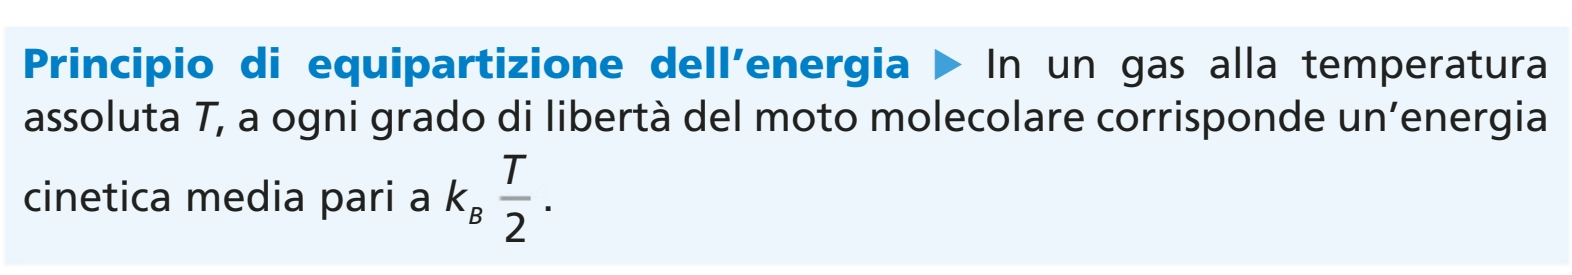
\includegraphics[width=0.88\linewidth]{immagini/box_equipartizione.jpg}
\caption{Riquadro didattico dal testo scolastico: il Principio di Equipartizione dell'Energia.}
\label{fig:equipartizione_box}
\end{figure}

\begin{leggefisica}[Principio di Equipartizione dell'Energia]
In un sistema termodinamico in equilibrio alla temperatura assoluta $T$, a ciascun grado di libertà indipendente del moto molecolare (traslazionale o rotazionale) compete un'energia cinetica media pari a:
\[
\langle E \rangle_1 = \frac{1}{2} \, k_B \, T
\]
Se una molecola possiede $l$ gradi di libertà attivi, l'energia cinetica media totale per molecola è:
\[
\mathbf{\langle K_{\text{tot}} \rangle = \frac{l}{2} \, k_B \, T}
\]
\end{leggefisica}

\begin{itemize}
  \item \textbf{Gas monoatomici (es. He, Ne, Ar):} 3 gradi di libertà traslazionali ($x, y, z$). $l = 3$:
  \[
  \langle K \rangle = \frac{3}{2} k_B T, \qquad U = \frac{3}{2} n R T
  \]
  \item \textbf{Gas biatomici (es. $N_2, O_2, H_2$ a temperatura ambiente):} 3 gradi di libertà traslazionali + 2 gradi di libertà rotazionali (rotazione attorno ai due assi ortogonali all'asse internucleare). $l = 5$:
  \[
  \langle K \rangle = \frac{5}{2} k_B T, \qquad U = \frac{5}{2} n R T
  \]
  \item \textbf{Gas poliatomici (es. $H_2O, CH_4$):} 3 traslazionali + 3 rotazionali attorno a tre assi indipendenti. $l = 6$:
  \[
  \langle K \rangle = 3 k_B T, \qquad U = 3 n R T
  \]
\end{itemize}

% ==============================================================================
% CAPITOLO 5
% ==============================================================================
\chapter{Lavoro Meccanico, Calore ed Equivalenza Termomeccanica}

Negli appunti di lezione (pagine 16--18), la trattazione fisica si amplia verso la termologia fondamentale e la genesi storica dell'equivalenza tra lavoro meccanico e calore, ponendo le basi microscopiche e macroscopiche del Primo Principio della Termodinamica.

\section{L'Esperimento del Mulinello di Joule ed Equivalenza Termomeccanica}
Fino alla met\`a del XIX secolo, il calore era considerato un fluido invisibile e imponderabile denominato \textbf{calorico}, capace di fluire spontaneamente dai corpi pi\`u caldi a quelli pi\`u freddi. Nel 1845 James Prescott Joule demol\`i tale impostazione teorica dimostrando che il calore non \`e una sostanza materiale, bens\`i una \textbf{forma di energia in transito} generata dalla dissipazione meccanica e dal lavoro delle forze di attrito viscoso.

Joule realizz\`o un calorimetro a pareti adiabatiche isolanti al cui interno era immersa una quantit\`a nota di acqua. Un albero centrale provvisto di palette rotanti era collegato tramite fili e carrucole a due corpi gravi di massa $m$ posti a un'altezza $h$ da terra.
\begin{center}
\begin{tikzpicture}[scale=0.9, >=stealth]
  % Trave di supporto
  \draw[thick, primaryBlue] (-3.5, 3.5) -- (3.5, 3.5);
  % Carrucola sinistra
  \draw[thick, fill=slateBorder!40] (-2.5, 3.5) circle (0.3);
  \draw[fill=primaryBlue] (-2.5, 3.5) circle (1.5pt);
  \draw[thick, slateBorder!120] (-2.8, 3.5) -- (-2.8, 1.8);
  \draw[thick, fill=primaryBlue!30] (-3.1, 1.2) rectangle (-2.5, 1.8);
  \node[font=\footnotesize\bfseries, primaryBlue] at (-2.8, 1.5) {$m$};
  \draw[->, thick, accentRed] (-3.4, 1.8) -- (-3.4, 1.0) node[midway, left, font=\scriptsize\bfseries] {$h, \, \vec{g}$};

  % Carrucola destra
  \draw[thick, fill=slateBorder!40] (2.5, 3.5) circle (0.3);
  \draw[fill=primaryBlue] (2.5, 3.5) circle (1.5pt);
  \draw[thick, slateBorder!120] (2.8, 3.5) -- (2.8, 1.8);
  \draw[thick, fill=primaryBlue!30] (2.5, 1.2) rectangle (3.1, 1.8);
  \node[font=\footnotesize\bfseries, primaryBlue] at (2.8, 1.5) {$m$};
  \draw[->, thick, accentRed] (3.4, 1.8) -- (3.4, 1.0) node[midway, right, font=\scriptsize\bfseries] {$h, \, \vec{g}$};

  % Cavi verso il tamburo centrale
  \draw[thick, slateBorder!120] (-2.2, 3.5) -- (-0.2, 2.7);
  \draw[thick, slateBorder!120] (2.2, 3.5) -- (0.2, 2.7);

  % Tamburo e asse centrale
  \draw[thick, fill=slateBorder!60] (-0.2, 2.5) rectangle (0.2, 2.9);
  \draw[ultra thick, primaryBlue] (0, 2.5) -- (0, -0.5);

  % Calorimetro (recipiente isolato)
  \draw[very thick, primaryBlue] (-1.8, 1.0) -- (-1.8, -1.5) -- (1.8, -1.5) -- (1.8, 1.0);
  \draw[thick, dashed, slateBorder] (-2.0, 1.2) -- (-2.0, -1.7) -- (2.0, -1.7) -- (2.0, 1.2);
  \fill[primaryBlue!15] (-1.75, 0.7) rectangle (1.75, -1.45);
  \node[font=\scriptsize\sffamily, primaryBlue] at (-1.0, 0.4) {Acqua ($m_w$)};

  % Palette rotanti sull'albero
  \draw[very thick, accentAmber] (-1.2, 0.0) -- (1.2, 0.0);
  \draw[very thick, accentAmber] (-1.2, -0.6) -- (1.2, -0.6);
  \draw[very thick, accentAmber] (-1.2, -1.1) -- (1.2, -1.1);
  \draw[->, thick, accentAmber] (0.5, 2.1) arc (0:220:0.5 and 0.2);
  \node[right, font=\scriptsize\bfseries, accentAmber] at (0.6, 2.1) {$\omega$};

  % Termometro
  \draw[thick, fill=white] (1.2, 1.8) -- (1.2, -0.8);
  \draw[thick, fill=white] (1.4, 1.8) -- (1.4, -0.8);
  \draw[fill=accentRed] (1.15, -0.8) rectangle (1.45, -1.2);
  \draw[thick, fill=accentRed] (1.3, -1.2) circle (0.2);
  \draw[line width=1.5pt, accentRed] (1.3, -1.0) -- (1.3, 0.8);
  \node[right, font=\scriptsize\bfseries, accentRed] at (1.5, 1.2) {Termometro ($\Delta T$)};

  % Didascalie energetiche
  \node[draw=primaryBlue, fill=white, rounded corners=2pt, font=\scriptsize\bfseries, align=center] at (-2.8, -0.3) {Lavoro gravitazionale:\\$W = 2\,mgh$};
  \node[draw=accentAmber, fill=white, rounded corners=2pt, font=\scriptsize\bfseries, align=center] at (0, -2.2) {Dissipazione per attrito viscoso:\\$Q = W \implies \mathbf{1\,\text{cal} \approx 4{,}186\,\text{J}}$};
\end{tikzpicture}
\par\vspace{1.5mm}{\small\textbf{Figura 5.1:} \textit{Apparato sperimentale del mulinello di Joule: le masse gravi $m$ scendono di una quota $h$, cedendo energia potenziale gravitazionale $W = 2mgh$. L'albero ruota vorticosamente e le palette dissipano l'energia per attrito viscoso nell'acqua, producendo un innalzamento termico $\Delta T$ misurato dal termometro.}}
\end{center}

Lasciando cadere i pesi, l'energia potenziale gravitazionale persa:
\[
W = 2 \, m \, g \, h
\]
viene interamente trasferita alle palette che, rimescolando l'acqua contro le resistenze viscose microscopiche, convertono il lavoro meccanico ordinato in moti molecolari caotici, producendo un incremento termico misurabile $\Delta T$.

\begin{leggefisica}[Equivalente Meccanico della Caloria]
Joule prov\`o che il rapporto tra il lavoro meccanico speso $W$ e la quantit\`a di calore $Q$ prodotta \`e rigorosamente costante:
\[
\mathbf{1\,\text{cal} = 4{,}186\,\text{J}} \qquad \left(1\,\text{kcal} = 4186\,\text{J}\right)
\]
La caloria non rappresenta dunque una grandezza indipendente, bens\`i un'unit\`a di misura tradizionale per quantificare l'energia interna scambiata.
\end{leggefisica}

\section{Capacit\`a Termica e Calore Specifico}
La quantit\`a di calore $Q$ che un corpo di massa $m$ deve assorbire o cedere per variare la propria temperatura di $\Delta T = T_f - T_i$ (oppure $\Delta t = t_f - t_i$) \`e regolata dalla \textbf{legge fondamentale della termologia}:
\[
\mathbf{Q = m \cdot c \cdot \Delta T = C \cdot \Delta T}
\]
dove:
\begin{itemize}
  \item $c$ \`e il \textbf{calore specifico} della sostanza, espresso nel Sistema Internazionale in $\text{J/(kg}\cdot\text{K)}$ (oppure in $\text{cal/(g}\cdot{^\circ}\text{C)}$). Esso misura l'inerzia termica della materia, cio\`e l'energia necessaria per innalzare di $1\,\text{K}$ la temperatura di $1\,\text{kg}$ di sostanza;
  \item $C = m \cdot c$ \`e la \textbf{capacit\`a termica} globale dell'oggetto, espressa in $\text{J/K}$.
\end{itemize}

\begin{table}[htbp]
\centering
\small
\begin{tabularx}{\linewidth}{l c c X}
\toprule
\textbf{Sostanza} & \textbf{$c$ [$\text{J/(kg}\cdot\text{K)}$]} & \textbf{$c$ [$\text{cal/(g}\cdot{^\circ}\text{C)}$]} & \textbf{Propriet\`a Didattica} \\
\midrule
Acqua liquida & $4186$ & $1{,}000$ & Straordinaria capacit\`a di accumulo termico (effetto volano climatico). \\
Alcol etilico & $2430$ & $0{,}580$ & Elevata volatilit\`a e capacit\`a termica intermedia. \\
Alluminio ($Al$) & $897$ & $0{,}214$ & Calore specifico doppio rispetto al ferro ($\approx 2 \times c_{Fe}$). \\
Ferro / Acciaio ($Fe$) & $448$ & $0{,}107$ & Moderata inerzia termica, rapido riscaldamento per conduzione. \\
Rame ($Cu$) & $387$ & $0{,}092$ & Eccellente conduttore termico per scambiatori ed ebollizione. \\
\bottomrule
\end{tabularx}
\caption{Valori di riferimento del calore specifico per sostanze di uso comune.}
\label{tab:calori_specifici}
\end{table}

\begin{commento}[Il Ruolo Termoregolatore dell'Acqua]
L'elevatissimo calore specifico dell'acqua ($c_{\text{acqua}} = 4186\,\text{J/(kg}\cdot\text{K)}$), circa dieci volte superiore a quello dei metalli comuni, spiega perch\'e le grandi masse d'acqua (mari e laghi) agiscano da imponenti stabilizzatori termici per il clima costiero: assorbono enormi quantit\`a di calore solare durante il giorno e la stagione estiva subendo modeste variazioni di temperatura, e rilasciano gradualmente tale energia durante la notte e l'inverno.
\end{commento}

\section{Conservazione dell'Energia e Temperatura di Equilibrio}
Quando due corpi a temperature differenti $T_1$ e $T_2$ ($T_1 < T_2$) vengono posti a contatto termico all'interno di un calorimetro adiabatico (recipiente isolato in cui $Q_{\text{ambiente}} = 0$), il flusso di calore prosegue spontaneamente dal corpo pi\`u caldo al corpo pi\`u freddo fino al raggiungimento dell'\textbf{equilibrio termico} alla temperatura finale comune $T_{\text{eq}}$:
\begin{center}
\begin{tikzpicture}[scale=0.95, >=stealth]
  % Recipiente calorimetrico
  \draw[line width=2pt, primaryBlue] (-2.5, 2.2) -- (-2.5, -0.5) -- (2.5, -0.5) -- (2.5, 2.2);
  \draw[line width=1pt, dashed, slateBorder] (-2.7, 2.4) -- (-2.7, -0.7) -- (2.7, -0.7) -- (2.7, 2.4);
  \node[font=\tiny\sffamily, slateBorder!120] at (0, -0.9) {Isolamento adiabatico ideale ($Q_{\text{esterno}} = 0$)};

  % Acqua 1 (fredda)
  \fill[primaryBlue!20] (-2.45, 0.8) rectangle (2.45, -0.45);
  \node[font=\footnotesize\bfseries, primaryBlue] at (-1.3, 0.2) {Massa $m_1$, Calore sp. $c_1$};
  \node[font=\scriptsize\bfseries, primaryBlue] at (-1.3, -0.15) {Temp. iniziale $T_1$ (Fredda)};

  % Corpo / Acqua 2 (calda) introdotta
  \draw[very thick, fill=accentRed!25] (0.3, 0.9) rectangle (2.1, 1.9);
  \node[font=\footnotesize\bfseries, accentRed] at (1.2, 1.55) {Massa $m_2$, Calore sp. $c_2$};
  \node[font=\scriptsize\bfseries, accentRed] at (1.2, 1.2) {Temp. iniziale $T_2 > T_1$};

  % Frecce di flusso termico
  \draw[->, ultra thick, accentAmber, decorate, decoration={snake, amplitude=1.5pt, pre length=3pt, post length=3pt}] (1.2, 0.85) -- (1.2, 0.0) node[midway, right, font=\footnotesize\bfseries, accentAmber] {$Q_{\text{ceduto}}$};
  \draw[->, ultra thick, primaryBlue, decorate, decoration={snake, amplitude=1.5pt, pre length=3pt, post length=3pt}] (-0.2, 0.0) -- (-0.8, 0.0) node[midway, above, font=\footnotesize\bfseries, primaryBlue] {$Q_{\text{assorbito}}$};

  % Termometro centrale
  \draw[thick, fill=white] (-0.1, 2.5) rectangle (0.1, 0.1);
  \fill[accentRed] (-0.15, 0.1) rectangle (0.15, -0.2);
  \draw[thick, fill=accentRed] (0, -0.2) circle (0.2);
  \draw[line width=2pt, accentRed] (0, 0.1) -- (0, 1.8);
  \node[above, font=\footnotesize\bfseries, accentRed, fill=white, inner sep=1pt] at (0, 2.6) {$T_{\text{eq}} = \frac{m_1 c_1 T_1 + m_2 c_2 T_2}{m_1 c_1 + m_2 c_2}$};
\end{tikzpicture}
\par\vspace{1.5mm}{\small\textbf{Figura 5.2:} \textit{Mescolamento adiabatico in calorimetro: il calore ceduto dal corpo a temperatura pi\`u alta compensa rigorosamente il calore assorbito dal corpo freddo ($Q_{\text{ced}} + Q_{\text{ass}} = 0$).}}
\end{center}

Per il principio di conservazione dell'energia termica:
\[
Q_{\text{assorbito}} + Q_{\text{ceduto}} = 0 \implies m_1 c_1 (T_{\text{eq}} - T_1) + m_2 c_2 (T_{\text{eq}} - T_2) = 0
\]
Sviluppando algebricamente i prodotti e raggruppando i termini contenenti $T_{\text{eq}}$:
\[
m_1 c_1 T_{\text{eq}} - m_1 c_1 T_1 + m_2 c_2 T_{\text{eq}} - m_2 c_2 T_2 = 0
\]
\[
T_{\text{eq}} (m_1 c_1 + m_2 c_2) = m_1 c_1 T_1 + m_2 c_2 T_2 \implies \mathbf{T_{\text{eq}} = \frac{m_1 c_1 T_1 + m_2 c_2 T_2}{m_1 c_1 + m_2 c_2}}
\]

Nel caso notevole in cui i corpi siano composti dalla \textbf{stessa sostanza} ($c_1 = c_2 = c$, come nel mescolamento di due quantit\`a d'acqua a temperature diverse descritto negli appunti a pagina 18):
\[
T_{\text{eq}} = \frac{c \, (m_1 T_1 + m_2 T_2)}{c \, (m_1 + m_2)} \implies \mathbf{T_{\text{eq}} = \frac{m_1 T_1 + m_2 T_2}{m_1 + m_2}}
\]
La temperatura finale \`e esattamente la \textbf{media ponderata} delle temperature iniziali pesata sulle rispettive masse.

\section{Il Kilowattora nei Consumi Energetici e nella Pratica Civile}
Nelle applicazioni civili, industriali e nella fatturazione dell'energia elettrica, l'unit\`a di misura del Sistema Internazionale (il Joule) risulta straordinariamente piccola. Si impiega pertanto il \textbf{Kilowattora} ($\text{kWh}$), definito come l'energia assorbita o erogata da un dispositivo della potenza costante di $1\,\text{kW}$ ($1000\,\text{W}$) per la durata di un'ora ($3600\,\text{s}$):
\[
\mathbf{1\,\text{kWh} = 1000\,\text{W} \times 3600\,\text{s} = 3{,}60 \cdot 10^6\,\text{J} = 3{,}60\,\text{MJ}}
\]
Come documentato negli appunti di lezione (pagina 17), l'energia assorbita da un'apparecchiatura elettrica si traduce in spesa monetaria: conoscendo il costo unitario dell'energia ($c_{\text{unit}} \approx 0{,}15\text{--}0{,}25\,\text{EUR/kWh}$), la spesa complessiva risulta:
\[
\text{Costo} = E_{[\text{kWh}]} \times c_{\text{unit}} = (P_{[\text{kW}]} \cdot \Delta t_{[\text{h}]}) \times c_{\text{unit}}
\]
% ==============================================================================
% CAPITOLO 6
% ==============================================================================
\chapter{Risoluzione Integrale dei Problemi del Testo Scolastico}

In questa sezione sono raccolti tutti e soli i problemi assegnati ed effettivamente svolti negli appunti di lezione. Ciascun problema riporta in apertura il ritaglio originale dal libro di testo scolastico per un immediato e inequivocabile riconoscimento, ed \`e svolto rigorosamente secondo il \textbf{Protocollo Canonico a 9 Fasi}. In conformit\`a con le direttive didattiche di fisica, la \textbf{Fase 4} \`e corredata per ciascun problema dallo \textbf{schema grafico vettoriale della situazione fisica} (\textit{disegnino analitico}), evidenziando corpi, vincoli, scambi termici e vettori di stato.

% ------------------------------------------------------------------------------
% PROBLEMA 1 (ESERCIZIO 15)
% ------------------------------------------------------------------------------
\section{Problema 1: Trasformazione Isoterma Reversibile e Piano $(V, p)$}

\begin{figure}[htbp]
\centering
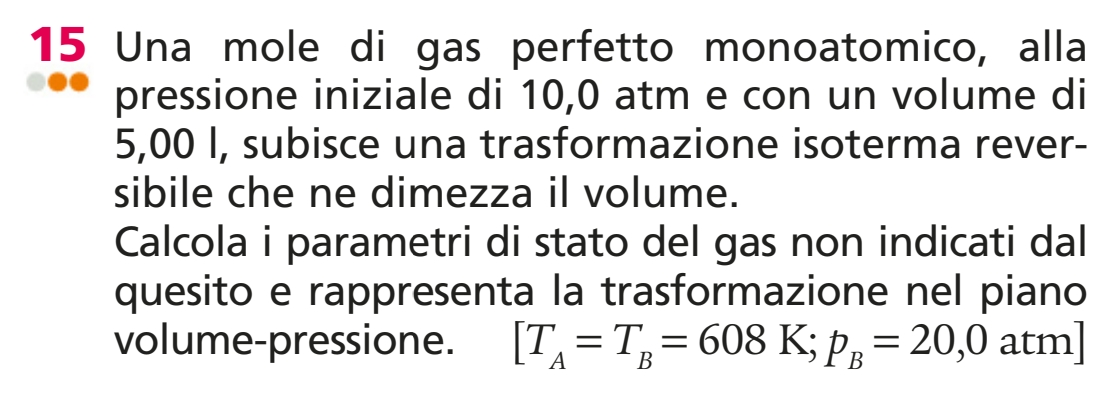
\includegraphics[width=0.85\linewidth]{immagini/es_15_traccia.jpg}
\caption{Traccia originale dal testo scolastico: Esercizio 15 (trasformazione isoterma).}
\label{fig:es15_testo}
\end{figure}

\begin{problema}[Esercizio 15: Risoluzione Strutturata a 9 Fasi]
\begin{enumerate}[label=\textbf{Fase \arabic*:}, leftmargin=*, itemsep=5pt]
  \item \textbf{Dati del Problema:}
  \begin{itemize}[leftmargin=*, label=\textbullet]
    \item Quantit\`a di sostanza: $n = 1{,}00\,\text{mol}$ (gas perfetto monoatomico);
    \item Pressione iniziale nello stato $A$: $p_A = 10{,}0\,\text{atm}$;
    \item Volume iniziale nello stato $A$: $V_A = 5{,}00\,\text{L}$;
    \item Trasformazione da $A$ a $B$: compressione isoterma quasi-statica reversibile ($T_A = T_B = \text{cost}$);
    \item Volume finale nello stato $B$: $V_B = \frac{V_A}{2} = 2{,}50\,\text{L}$.
  \end{itemize}

  \item \textbf{Incognite Formalizzate:}
  \begin{itemize}[leftmargin=*, label=\textbullet]
    \item Temperatura assoluta del gas: $T_A = T_B = ?\,\text{[K]}$;
    \item Pressione finale nello stato compresso $B$: $p_B = ?\,\text{[atm]}$;
    \item Traiettoria termodinamica analitica nel piano di Clapeyron $(V, p)$.
  \end{itemize}

  \item \textbf{Conversione nel Sistema Internazionale (SI):}
  \begin{itemize}[leftmargin=*, label=\textbullet]
    \item $p_A = 10{,}0\,\text{atm} = 10{,}0 \cdot 101325\,\text{Pa} = 1{,}01325 \cdot 10^6\,\text{Pa}$;
    \item $V_A = 5{,}00\,\text{L} = 5{,}00 \cdot 10^{-3}\,\text{m}^3$;
    \item $V_B = 2{,}50\,\text{L} = 2{,}50 \cdot 10^{-3}\,\text{m}^3$;
    \item Costante universale dei gas: $R = 8{,}314\,\text{J/(mol}\cdot\text{K)}$ (oppure $R = 0{,}0821\,\text{L}\cdot\text{atm/(mol}\cdot\text{K)}$).
  \end{itemize}

  \item \textbf{Modello Fisico e Schema della Situazione:}
  Modellizziamo il sistema come gas ideale confinato all'interno di un cilindro termicamente conduttore a contatto con un termostato (bagno termico a temperatura costante $T$). Una forza esterna $\vec{F}_{\text{ext}}$ applicata al pistone comprime lentamente il gas fino a dimezzarne il volume.
  \begin{center}
  \begin{tikzpicture}[scale=0.88, >=stealth]
    % Cilindro e pistone - Stato A (Iniziale)
    \begin{scope}[shift={(0,0)}]
      \draw[very thick, primaryBlue] (0,3.2) -- (0,0) -- (2.4,0) -- (2.4,3.2);
      \fill[primaryBlue!15] (0.05,0.05) rectangle (2.35,2.4);
      \foreach \pos in {(0.4,0.5), (1.2,0.8), (1.8,0.4), (0.7,1.5), (1.5,1.7), (2.0,1.2), (0.5,2.0), (1.1,2.2)} {
        \fill[primaryBlue] \pos circle (1.5pt);
      }
      \fill[slateBorder!70] (0.05,2.4) rectangle (2.35,2.7);
      \draw[thick, slateBorder!120] (0.05,2.4) rectangle (2.35,2.7);
      \draw[ultra thick, slateBorder!120] (1.2,2.7) -- (1.2,3.6);
      \draw[ultra thick, slateBorder!120] (0.7,3.6) -- (1.7,3.6);
      \draw[<->, thick, primaryBlue] (-0.3,0) -- (-0.3,2.4) node[midway, left, font=\footnotesize\bfseries] {$V_A = 5{,}0\,\text{L}$};
      \fill[accentAmber!25] (-0.2,-0.5) rectangle (2.6,0);
      \draw[thick, accentAmber] (-0.2,-0.5) rectangle (2.6,0);
      \node[font=\scriptsize\bfseries, accentAmber!90!black] at (1.2,-0.25) {Bagno $T = 608\,\text{K}$};
      \node[draw=primaryBlue, fill=white, rounded corners=2pt, font=\scriptsize\bfseries, primaryBlue, align=center] at (1.2,4.1) {STATO $A$ (Iniziale)\\$p_A = 10{,}0\,\text{atm}$};
    \end{scope}

    \draw[->, ultra thick, accentAmber] (3.0,1.8) -- (4.2,1.8) node[midway, above, font=\scriptsize\bfseries, align=center] {Compressione\\Isoterma};
    \node[below, font=\tiny\sffamily, slateBorder] at (3.6,1.6) {$T = \text{cost}$};

    % Cilindro e pistone - Stato B (Compresso)
    \begin{scope}[shift={(4.8,0)}]
      \draw[very thick, primaryBlue] (0,3.2) -- (0,0) -- (2.4,0) -- (2.4,3.2);
      \fill[accentRed!20] (0.05,0.05) rectangle (2.35,1.2);
      \foreach \pos in {(0.3,0.3), (0.8,0.5), (1.3,0.3), (1.9,0.4), (0.5,0.9), (1.1,0.8), (1.6,1.0), (2.1,0.8)} {
        \fill[accentRed] \pos circle (1.5pt);
      }
      \fill[slateBorder!70] (0.05,1.2) rectangle (2.35,1.5);
      \draw[thick, slateBorder!120] (0.05,1.2) rectangle (2.35,1.5);
      \draw[ultra thick, slateBorder!120] (1.2,1.5) -- (1.2,2.8);
      \draw[ultra thick, slateBorder!120] (0.7,2.8) -- (1.7,2.8);
      \draw[->, line width=1.5pt, accentRed] (1.2,3.5) -- (1.2,2.9) node[above, font=\scriptsize\bfseries] {$\vec{F}_{\text{ext}}$};
      \draw[<->, thick, accentRed] (-0.3,0) -- (-0.3,1.2) node[midway, left, font=\footnotesize\bfseries] {$V_B = 2{,}5\,\text{L}$};
      \fill[accentAmber!25] (-0.2,-0.5) rectangle (2.6,0);
      \draw[thick, accentAmber] (-0.2,-0.5) rectangle (2.6,0);
      \node[font=\scriptsize\bfseries, accentAmber!90!black] at (1.2,-0.25) {Bagno $T = 608\,\text{K}$};
      \node[draw=accentRed, fill=white, rounded corners=2pt, font=\scriptsize\bfseries, accentRed, align=center] at (1.2,4.1) {STATO $B$ (Compresso)\\$p_B = 20{,}0\,\text{atm}$};
    \end{scope}
  \end{tikzpicture}
  \par\vspace{1.5mm}{\small\textbf{Figura 6.2:} \textit{Schema della situazione fisica dell'Esercizio 15: compressione quasi-statica del cilindro a contatto con il bagno termico a $T = 608\,\text{K}$. Al dimezzarsi del volume ($V_B = V_A/2$), la frequenza degli urti molecolari e la pressione raddoppiano ($p_B = 2p_A$).}}
  \end{center}

  \item \textbf{Leggi Fisiche Fondamentali in Forma Simbolica:}
  Dall'equazione di stato dei gas ideali per lo stato iniziale $A$:
  \[
  p_A V_A = n R T \implies T = \frac{p_A V_A}{n R}
  \]
  Dalla Legge di Boyle-Mariotte per trasformazioni isoterme reversibili ($T = \text{cost}$):
  \[
  p_A V_A = p_B V_B = \text{costante}
  \]

  \item \textbf{Risoluzione Algebrica Simbolica Letterale:}
  Isoliamo l'incognita $p_B$ prima di sostituire i valori numerici:
  \[
  p_B = p_A \, \frac{V_A}{V_B}
  \]
  Essendo $V_B = \frac{V_A}{2}$, si ottiene:
  \[
  p_B = p_A \, \frac{V_A}{\frac{V_A}{2}} = 2 \, p_A
  \]

  \item \textbf{Sostituzione Numerica Finale:}
  Calcoliamo la pressione finale:
  \[
  p_B = 2 \cdot 10{,}0\,\text{atm} = \mathbf{20{,}0\,\text{atm}} = 2{,}0265 \cdot 10^6\,\text{Pa}
  \]
  Calcoliamo la temperatura assoluta:
  \[
  T = \frac{(1{,}01325 \cdot 10^6\,\text{Pa}) \cdot (5{,}00 \cdot 10^{-3}\,\text{m}^3)}{1{,}00\,\text{mol} \cdot 8{,}314\,\text{J/(mol}\cdot\text{K)}} = \frac{5066{,}25}{8{,}314} \approx \mathbf{608\,\text{K}}
  \]

  \item \textbf{Risultato Riquadrato con Unit\`a e Cifre Significative:}
  \[
  \mathbf{\boxed{T_A = T_B \approx 608\,\text{K}}} \qquad \text{e} \qquad \mathbf{\boxed{p_B = 20{,}0\,\text{atm} \approx 2{,}03 \cdot 10^6\,\text{Pa}}}
  \]

  \item \textbf{Valutazione di Plausibilit\`a Fisica e Casi Limite:}
  \begin{itemize}[leftmargin=*, label=\textbullet]
    \item \textit{Verifica dimensionale:} $\left[\frac{p V}{n R}\right] = \frac{\text{Pa}\cdot\text{m}^3}{\text{mol}\cdot(\text{J}/(\text{mol}\cdot\text{K}))} = \frac{\text{J}}{\text{J/K}} = \text{K}$, coerente.
    \item \textit{Plausibilit\`a fisica:} Il raddoppio della pressione a seguito del dimezzamento del volume a temperatura costante riflette esattamente la legge di proporzionalit\`a inversa di Boyle.
    \item \textit{Casi limite:} Se $V_B \to V_A$, allora $p_B \to p_A$ (trasformazione nulla); se $V_B \to 0$, $p_B \to \infty$ (incomprimibilit\`a limite del volume nullo).
  \end{itemize}
\end{enumerate}
\end{problema}

\begin{figure}[htbp]
\centering
\begin{tikzpicture}[scale=1.1]
  \draw[step=1cm, slateBorder!40, very thin] (0,0) grid (7,5.5);
  \draw[->, thick, primaryBlue] (0,0) -- (7.2,0) node[below right, font=\small\sffamily] {$V \, [\text{L}]$};
  \draw[->, thick, primaryBlue] (0,0) -- (0,5.5) node[above left, font=\small\sffamily] {$p \, [\text{atm}]$};
  \draw[thick] (2.5, 0.1) -- (2.5, -0.1) node[below, font=\footnotesize] {$2{,}50$};
  \draw[thick] (5.0, 0.1) -- (5.0, -0.1) node[below, font=\footnotesize] {$5{,}00$};
  \draw[thick] (0.1, 2.0) -- (-0.1, 2.0) node[left, font=\footnotesize] {$10{,}0$};
  \draw[thick] (0.1, 4.0) -- (-0.1, 4.0) node[left, font=\footnotesize] {$20{,}0$};
  \draw[dashed, slateBorder] (5.0, 0) -- (5.0, 2.0) -- (0, 2.0);
  \draw[dashed, slateBorder] (2.5, 0) -- (2.5, 4.0) -- (0, 4.0);
  \draw[very thick, primaryBlue, domain=2.0:6.5, samples=100] plot (\x, {10.0/\x});
  \draw[-{Latex[length=3mm]}, very thick, accentAmber] (4.0, 2.5) -- (3.2, 3.125) node[midway, above right, font=\footnotesize\bfseries, fill=white, inner sep=1pt] {Compressione};
  \fill[accentGreen] (5.0, 2.0) circle (3pt);
  \node[above right, font=\footnotesize\bfseries, fill=white, fill opacity=0.9, text opacity=1, inner sep=2pt] at (5.0, 2.0) {$A(5{,}00\,\text{L}; 10{,}0\,\text{atm})$};
  \fill[accentRed] (2.5, 4.0) circle (3pt);
  \node[above right, font=\footnotesize\bfseries, fill=white, fill opacity=0.9, text opacity=1, inner sep=2pt] at (2.5, 4.0) {$B(2{,}50\,\text{L}; 20{,}0\,\text{atm})$};
  \node[font=\footnotesize\sffamily, primaryBlue, fill=white, inner sep=1pt] at (5.6, 1.2) {Isoterma $T = 608\,\text{K}$ (Iperbole equilatera $p \cdot V = 50\,\text{L}\cdot\text{atm}$)};
\end{tikzpicture}
\caption{Grafico cartesiano analitico dell'Esercizio 15: trasformazione isoterma $A \to B$ sul piano di Clapeyron (ramo di iperbole equilatera asintotico agli assi cartesiani $V=0$ e $p=0$).}
\label{fig:clapeyron_es15}
\end{figure}

% ------------------------------------------------------------------------------
% PROBLEMA 2 (ESERCIZIO 26)
% ------------------------------------------------------------------------------
\newpage
\section{Problema 2: Pressione dell'Idrogeno Calcolata dalla Densit\`a Volumica}

\begin{figure}[htbp]
\centering
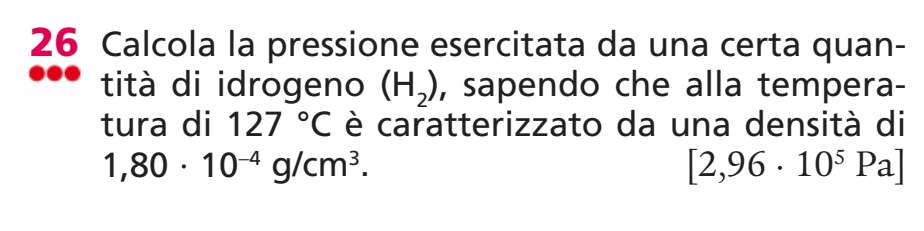
\includegraphics[width=0.85\linewidth]{immagini/es_26_traccia.jpg}
\caption{Traccia originale dal testo scolastico: Esercizio 26 (densit\`a dell'idrogeno).}
\label{fig:es26_testo}
\end{figure}

\begin{problema}[Esercizio 26: Risoluzione Strutturata a 9 Fasi]
\begin{enumerate}[label=\textbf{Fase \arabic*:}, leftmargin=*, itemsep=5pt]
  \item \textbf{Dati del Problema:}
  \begin{itemize}[leftmargin=*, label=\textbullet]
    \item Sostanza: Idrogeno molecolare $H_2$ ($M = 2 \cdot 1{,}008\,\text{g/mol} = 2{,}016\,\text{g/mol}$);
    \item Temperatura centigrada: $t = 127\,{^\circ}\text{C}$;
    \item Densit\`a volumica di massa del gas: $\rho = 1{,}80 \cdot 10^{-4}\,\text{g/cm}^3$;
    \item Costante universale dei gas: $R = 8{,}314\,\text{J/(mol}\cdot\text{K)}$.
  \end{itemize}

  \item \textbf{Incognite Formalizzate:}
  \begin{itemize}[leftmargin=*, label=\textbullet]
    \item Pressione macroscopica $p$ esercitata dal gas in Pascal ($\text{Pa}$) e in atmosfere ($\text{atm}$).
  \end{itemize}

  \item \textbf{Conversione nel Sistema Internazionale (SI):}
  \begin{itemize}[leftmargin=*, label=\textbullet]
    \item $T = t + 273{,}15 = 127 + 273{,}15 = 400{,}15\,\text{K}$;
    \item $\rho = 1{,}80 \cdot 10^{-4}\,\frac{\text{g}}{\text{cm}^3} = 1{,}80 \cdot 10^{-4} \cdot \frac{10^{-3}\,\text{kg}}{10^{-6}\,\text{m}^3} = 0{,}180\,\text{kg/m}^3$;
    \item Massa molare: $M = 2{,}016 \cdot 10^{-3}\,\text{kg/mol}$.
  \end{itemize}

  \item \textbf{Modello Fisico e Schema della Situazione:}
  Rappresentiamo il gas come insieme di molecole biatomiche $H_2$ racchiuse in un volume $V$. A livello microscopico, ciascuna molecola che urta elasticamente la parete con componente normale $v_x$ subisce una variazione della quantit\`a di moto pari a $\Delta p_x = -2mv_x$. Per l'insieme delle particelle di massa totale $m = \rho V$, l'effetto collettivo degli urti microscopici determina la pressione macroscopica stazionaria $p$.
  \begin{center}
  \begin{tikzpicture}[scale=0.92, >=stealth]
    \fill[gray!20] (5, -0.2) rectangle (5.3, 3.2);
    \draw[very thick, slateBorder!120] (5, -0.2) -- (5, 3.2);
    \draw[thick, gray!60] (0, 0) -- (5, 0);
    \draw[thick, gray!60] (0, 3) -- (5, 3);
    \draw[thick, gray!60] (0, 0) -- (0, 3);

    \node[font=\scriptsize\sffamily, slateBorder] at (1.4, 2.7) {Gas $H_2$ ($\rho = 0{,}180\,\text{kg/m}^3$)};
    \node[font=\scriptsize\sffamily, slateBorder] at (1.4, 2.3) {$T = 400{,}15\,\text{K}$ ($127^\circ\text{C}$)};

    \foreach \x/\y in {0.8/0.6, 1.5/1.4, 2.2/0.7, 1.0/1.9, 3.0/2.2, 3.8/0.9, 2.5/1.7} {
      \fill[primaryBlue!40] (\x, \y) circle (2pt);
      \fill[primaryBlue!40] (\x+0.08, \y+0.08) circle (2pt);
      \draw[primaryBlue, ultra thin] (\x, \y) -- (\x+0.08, \y+0.08);
    }

    \coordinate (col) at (5, 1.5);
    \draw[dashed, primaryBlue, thick] (3.0, 0.7) -- (col);
    \draw[->, very thick, primaryBlue] (3.0, 0.7) -- (4.2, 1.18) node[midway, below right, font=\footnotesize] {$\vec{v}_{\text{in}}$};
    \fill[primaryBlue] (3.0, 0.7) circle (2.5pt);

    \draw[dashed, accentRed, thick] (col) -- (3.0, 2.3);
    \draw[->, very thick, accentRed] (col) -- (3.8, 1.98) node[midway, above right, font=\footnotesize] {$\vec{v}_{\text{fin}}$};
    \fill[accentRed] (3.8, 1.98) circle (2.5pt);

    \draw[->, thick, black] (col) -- (6.0, 1.5) node[right, font=\footnotesize] {$\hat{n}$};
    \draw[->, line width=1.8pt, accentAmber] (col) -- (3.8, 1.5) node[left, font=\footnotesize\bfseries] {$\Delta \vec{p}_x = -2mv_x$};
    \draw[->, line width=2pt, accentGreen!80!black] (5.0, 0.8) -- (5.8, 0.8) node[right, font=\footnotesize\bfseries] {$\vec{F}_{\text{parete}}$};

    \node[draw=primaryBlue, fill=white, rounded corners=3pt, font=\scriptsize\bfseries, align=center] at (2.5, -0.6) {Relazione macroscopica: $p = \dfrac{\rho R T}{M} \approx \mathbf{2{,}96 \cdot 10^5\,\text{Pa}}$};
  \end{tikzpicture}
  \par\vspace{1.5mm}{\small\textbf{Figura 6.5:} \textit{Schema cinetico dell'Esercizio 26: urto elastico della molecola di idrogeno $H_2$ contro la parete. L'inversione della quantit\`a di moto microscopica genera la forza media e la pressione macroscopica $p = \frac{\rho R T}{M}$.}}
  \end{center}

  \item \textbf{Leggi Fisiche Fondamentali in Forma Simbolica:}
  Dall'equazione di stato dei gas perfetti:
  \[
  p V = n R T
  \]
  Esprimendo il numero di moli come $n = \frac{m}{M}$ e la densit\`a di massa come $\rho = \frac{m}{V}$:
  \[
  p V = \frac{m}{M} \, R \, T
  \]

  \item \textbf{Risoluzione Algebrica Simbolica Letterale:}
  Dividendo ambo i membri per il volume $V$ e raccogliendo il rapporto $\frac{m}{V} = \rho$:
  \[
  p = \left(\frac{m}{V}\right) \frac{R \, T}{M} \implies \mathbf{p = \frac{\rho \cdot R \cdot T}{M}}
  \]

  \item \textbf{Sostituzione Numerica Finale:}
  Sostituendo i valori nel Sistema Internazionale:
  \[
  p = \frac{(0{,}180\,\text{kg/m}^3) \cdot (8{,}314\,\text{J/(mol}\cdot\text{K)}) \cdot (400{,}15\,\text{K})}{2{,}016 \cdot 10^{-3}\,\text{kg/mol}} = \frac{598{,}83}{2{,}016 \cdot 10^{-3}} \approx \mathbf{2{,}96 \cdot 10^5\,\text{Pa}}
  \]
  In atmosfere:
  \[
  p = \frac{2{,}96 \cdot 10^5\,\text{Pa}}{101325\,\text{Pa/atm}} \approx \mathbf{2{,}92\,\text{atm}}
  \]

  \item \textbf{Risultato Riquadrato con Unit\`a e Cifre Significative:}
  \[
  \mathbf{\boxed{p \approx 2{,}96 \cdot 10^5\,\text{Pa} \approx 2{,}92\,\text{atm}}}
  \]

  \item \textbf{Valutazione di Plausibilit\`a Fisica e Casi Limite:}
  \begin{itemize}[leftmargin=*, label=\textbullet]
    \item \textit{Verifica dimensionale:} $\left[\frac{\rho R T}{M}\right] = \frac{(\text{kg/m}^3) \cdot (\text{J}/(\text{mol}\cdot\text{K})) \cdot \text{K}}{\text{kg/mol}} = \frac{\text{J}}{\text{m}^3} = \frac{\text{N}\cdot\text{m}}{\text{m}^3} = \frac{\text{N}}{\text{m}^2} = \text{Pa}$, corretta.
    \item \textit{Plausibilit\`a fisica:} Circa $2{,}9\,\text{atm}$ \`e una pressione del tutto realistica per un gas leggero e molto riscaldato ($127^\circ\text{C}$).
    \item \textit{Casi limite:} Per $\rho \to 0$ (vuoto) si ha $p \to 0$; per $T \to 0$ (zero assoluto) si ha $p \to 0$, coerentemente con l'assenza di agitazione termica.
  \end{itemize}
\end{enumerate}
\end{problema}

% ------------------------------------------------------------------------------
% PROBLEMA 3 (ESERCIZIO 16)
% ------------------------------------------------------------------------------
\newpage
\section{Problema 3: Trasformazione Isocora e Sovrapressione in un Serbatoio}

\begin{figure}[htbp]
\centering
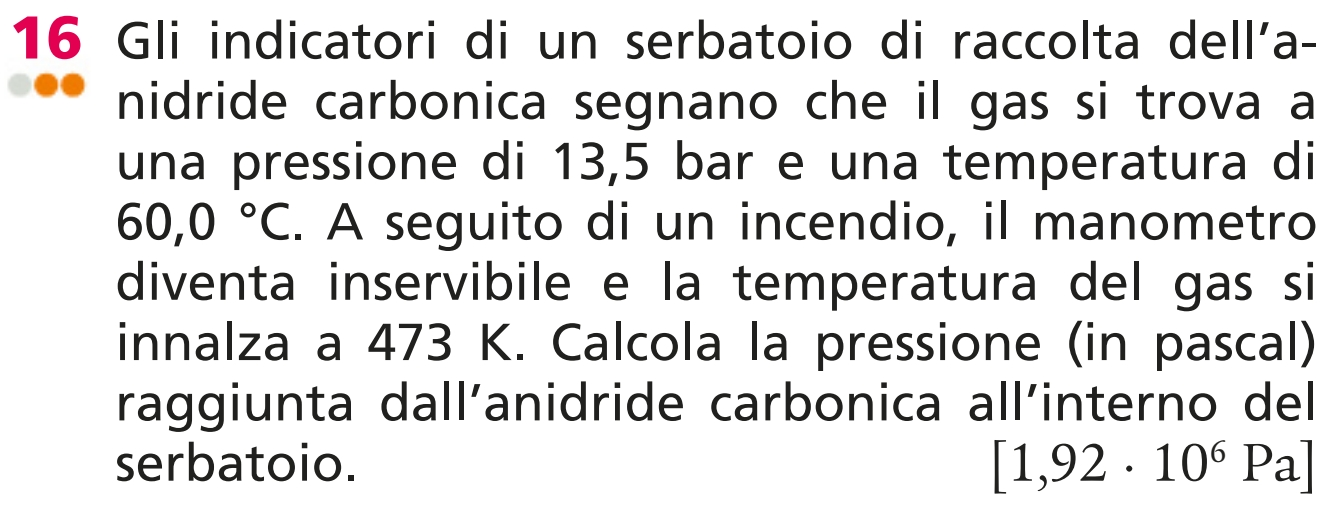
\includegraphics[width=0.85\linewidth]{immagini/es_16_traccia.jpg}
\caption{Traccia originale dal testo scolastico: Esercizio 16 (serbatoio rigido durante incendio).}
\label{fig:es16_testo}
\end{figure}

\begin{problema}[Esercizio 16: Risoluzione Strutturata a 9 Fasi]
\begin{enumerate}[label=\textbf{Fase \arabic*:}, leftmargin=*, itemsep=5pt]
  \item \textbf{Dati del Problema:}
  \begin{itemize}[leftmargin=*, label=\textbullet]
    \item Pressione iniziale del gas: $p_1 = 13{,}5\,\text{bar}$;
    \item Temperatura iniziale: $t_1 = 60{,}0\,{^\circ}\text{C}$;
    \item Temperatura finale durante l'incendio: $T_2 = 473\,\text{K}$;
    \item Vincolo geometrico: serbatoio metallico rigido indeformabile ($V = \text{costante}$).
  \end{itemize}

  \item \textbf{Incognite Formalizzate:}
  \begin{itemize}[leftmargin=*, label=\textbullet]
    \item Pressione finale $p_2$ raggiunta dall'anidride carbonica ($CO_2$) in $\text{Pa}$ e $\text{bar}$;
    \item Incremento percentuale di sovrapressione $\frac{\Delta p}{p_1} \cdot 100\%$.
  \end{itemize}

  \item \textbf{Conversione nel Sistema Internazionale (SI):}
  \begin{itemize}[leftmargin=*, label=\textbullet]
    \item $p_1 = 13{,}5\,\text{bar} = 13{,}5 \cdot 10^5\,\text{Pa} = 1{,}35 \cdot 10^6\,\text{Pa}$;
    \item $T_1 = 60{,}0 + 273{,}15 = 333{,}15\,\text{K}$;
    \item $T_2 = 473\,\text{K}$ (gi\`a espressa in Kelvin).
  \end{itemize}

  \item \textbf{Modello Fisico e Schema della Situazione:}
  Il sistema \`e modellato come un volume chiuso e indeformabile di gas ($V = \text{cost}$). Durante l'incendio, l'apporto termico per conduzione e irraggiamento $Q$ innalza l'energia cinetica media delle molecole, provocando un aumento proporzionale della quantit\`a di moto trasferita per unit\`a di superficie alle pareti metalliche del serbatoio.
  \begin{center}
  \begin{tikzpicture}[scale=0.88, >=stealth]
    \fill[slateBorder!20] (-0.3, -0.3) rectangle (3.3, 4.3);
    \fill[white] (0, 0) rectangle (3.0, 4.0);
    \draw[line width=2.5pt, slateBorder!120] (0, 4.0) -- (0, 0) -- (3.0, 0) -- (3.0, 4.0);
    \draw[line width=2.5pt, slateBorder!120] (0, 4.0) -- (1.1, 4.0);
    \draw[line width=2.5pt, slateBorder!120] (1.9, 4.0) -- (3.0, 4.0);

    \node[font=\footnotesize\bfseries, slateBorder!120] at (1.5, 3.5) {$V = \text{costante}$};
    \node[font=\scriptsize, slateBorder] at (1.5, 3.1) {Gas $CO_2$ confinato};

    \foreach \x in {0.2, 0.6, 1.0, 1.4, 1.8, 2.2, 2.6} {
      \draw[accentRed, fill=accentAmber, thick] (\x, -0.4) .. controls (\x-0.1, -0.1) and (\x, 0.1) .. (\x+0.1, -0.1) .. controls (\x+0.2, 0.2) .. (\x+0.2, -0.4) -- cycle;
    }
    \node[below, font=\scriptsize\bfseries, accentRed] at (1.5, -0.5) {INCENDIO: $Q_{\text{assorbito}} \implies T_1(333\,\text{K}) \to T_2(473\,\text{K})$};

    \draw[->, line width=1.5pt, accentRed] (1.5, 2.0) -- (0.2, 2.0);
    \draw[->, line width=1.5pt, accentRed] (1.5, 2.0) -- (2.8, 2.0);
    \draw[->, line width=1.5pt, accentRed] (1.5, 2.0) -- (1.5, 0.3);
    \draw[->, line width=1.5pt, accentRed] (1.5, 2.0) -- (1.5, 3.7);
    \draw[->, line width=1.2pt, accentRed] (1.5, 2.0) -- (0.5, 0.8);
    \draw[->, line width=1.2pt, accentRed] (1.5, 2.0) -- (2.5, 0.8);
    \draw[->, line width=1.2pt, accentRed] (1.5, 2.0) -- (0.5, 3.2);
    \draw[->, line width=1.2pt, accentRed] (1.5, 2.0) -- (2.5, 3.2);

    \draw[line width=1.5pt, slateBorder!120] (1.5, 4.0) -- (1.5, 4.5);
    \fill[white, draw=primaryBlue, line width=1.5pt] (1.5, 5.2) circle (0.7);
    \draw[thick, gray!50] (1.0, 5.2) arc (180:0:0.5);
    \draw[->, line width=1.5pt, accentRed] (1.5, 5.2) -- (1.85, 5.55);
    \node[font=\tiny\bfseries, slateBorder] at (1.5, 4.8) {bar};
    \node[font=\tiny, primaryBlue] at (1.1, 5.3) {$13{,}5$};
    \node[font=\tiny, accentRed] at (1.9, 5.3) {$19{,}2$};

    \node[draw=accentRed, fill=white, rounded corners=3pt, font=\scriptsize\bfseries, accentRed, align=left] at (5.5, 2.0) {
      \textbf{Aumento Termico Isocoro:}\\
      $p_2 = p_1 \cdot \dfrac{T_2}{T_1}$\\[1mm]
      $p_1 = 13{,}5\,\text{bar} \to \mathbf{p_2 = 19{,}2\,\text{bar}}$\\[1mm]
      $\Delta p = +5{,}7\,\text{bar}$ (\textbf{+42\% di sovrapressione})\\
      \textit{Rischio esplosione senza valvola!}
    };
  \end{tikzpicture}
  \par\vspace{1.5mm}{\small\textbf{Figura 6.7:} \textit{Schema fisico dell'Esercizio 16: riscaldamento isocoro ($V = \text{cost}$) di un serbatoio rigido durante un incendio. L'incremento di temperatura da $333{,}15\,\text{K}$ a $473\,\text{K}$ porta la pressione interna da $13{,}5\,\text{bar}$ a $19{,}2\,\text{bar}$ ($+42\%$).}}
  \end{center}

  \item \textbf{Leggi Fisiche Fondamentali in Forma Simbolica:}
  Per una trasformazione isocora reversibile di un gas ideale si applica la Seconda Legge di Gay-Lussac:
  \[
  \frac{p}{T} = \text{costante} \implies \frac{p_1}{T_1} = \frac{p_2}{T_2}
  \]

  \item \textbf{Risoluzione Algebrica Simbolica Letterale:}
  Isolando la pressione finale incognita $p_2$:
  \[
  \mathbf{p_2 = p_1 \cdot \frac{T_2}{T_1}}
  \]

  \item \textbf{Sostituzione Numerica Finale:}
  Sostituendo i valori numerici:
  \[
  p_2 = (1{,}35 \cdot 10^6\,\text{Pa}) \cdot \frac{473\,\text{K}}{333{,}15\,\text{K}} \approx 1{,}917 \cdot 10^6\,\text{Pa} = \mathbf{19{,}2\,\text{bar}}
  \]
  Incremento relativo di pressione:
  \[
  \frac{\Delta p}{p_1} = \frac{19{,}17 - 13{,}5}{13{,}5} = \frac{5{,}67}{13{,}5} \approx +42{,}0\%
  \]

  \item \textbf{Risultato Riquadrato con Unit\`a e Cifre Significative:}
  \[
  \mathbf{\boxed{p_2 \approx 1{,}92 \cdot 10^6\,\text{Pa} = 19{,}2\,\text{bar}}}
  \]

  \item \textbf{Valutazione di Plausibilit\`a Fisica e Casi Limite:}
  \begin{itemize}[leftmargin=*, label=\textbullet]
    \item \textit{Verifica dimensionale:} $\left[p_1 \cdot \frac{T_2}{T_1}\right] = \text{bar} \cdot \frac{\text{K}}{\text{K}} = \text{bar}$ (oppure $\text{Pa}$), coerente.
    \item \textit{Plausibilit\`a fisica e sicurezza:} L'aumento del $+42\%$ della pressione ($+5{,}7\,\text{bar}$) evidenzia il gravissimo rischio di scoppio per serbatoi a volume bloccato durante un incendio, confermando l'assoluta necessit\`a di valvole di sfiato tarate.
    \item \textit{Casi limite:} Se $T_2 = T_1$, allora $p_2 = p_1$ (equilibrio termico); se $T_2 \to 0\,\text{K}$, $p_2 \to 0$ (pressione nulla allo zero assoluto).
  \end{itemize}
\end{enumerate}
\end{problema}

% ------------------------------------------------------------------------------
% PROBLEMA 4 (ESERCIZIO 42)
% ------------------------------------------------------------------------------
\newpage
\section{Problema 4: Modello Dinamico della Pressione — Urti di Chicchi di Grandine}

\begin{figure}[htbp]
\centering
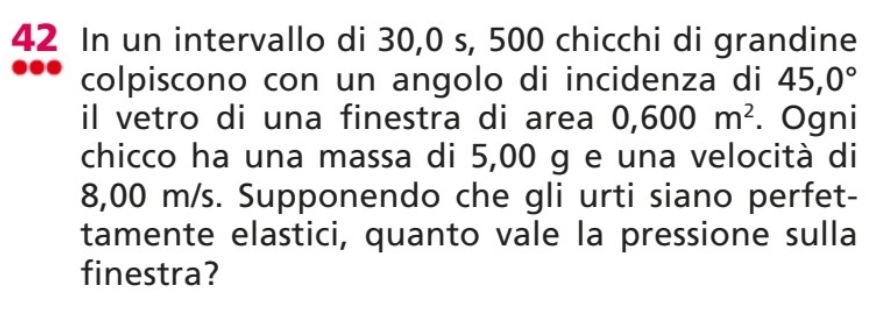
\includegraphics[width=0.85\linewidth]{immagini/es_42_traccia.jpg}
\caption{Traccia originale dal testo scolastico: Esercizio 42 (urti di chicchi di grandine).}
\label{fig:es42_testo}
\end{figure}

\begin{problema}[Esercizio 42: Risoluzione Strutturata a 9 Fasi]
\begin{enumerate}[label=\textbf{Fase \arabic*:}, leftmargin=*, itemsep=5pt]
  \item \textbf{Dati del Problema:}
  \begin{itemize}[leftmargin=*, label=\textbullet]
    \item Intervallo di tempo di osservazione: $\Delta t = 30{,}0\,\text{s}$;
    \item Numero totale di chicchi che colpiscono la superficie: $N = 500$;
    \item Angolo di incidenza rispetto alla normale della superficie: $\theta = 45{,}0^\circ$;
    \item Area della finestra: $A = 0{,}600\,\text{m}^2$;
    \item Massa di ciascun chicco di grandine: $m = 5{,}00\,\text{g}$;
    \item Velocit\`a del chicco incidente: $v = 8{,}00\,\text{m/s}$ (ipotesi di urti perfettamente elastici).
  \end{itemize}

  \item \textbf{Incognite Formalizzate:}
  \begin{itemize}[leftmargin=*, label=\textbullet]
    \item Impulso totale normale trasmesso alla finestra: $J_{\text{tot}} = ?\,\text{[N}\cdot\text{s]}$;
    \item Forza media complessiva impressa: $F_{\text{media}} = ?\,\text{[N]}$;
    \item Pressione media esercitata sulla finestra: $p = ?\,\text{[Pa]}$.
  \end{itemize}

  \item \textbf{Conversione nel Sistema Internazionale (SI):}
  \begin{itemize}[leftmargin=*, label=\textbullet]
    \item $m = 5{,}00\,\text{g} = 5{,}00 \cdot 10^{-3}\,\text{kg}$;
    \item $\cos(45{,}0^\circ) = \frac{\sqrt{2}}{2} \approx 0{,}7071$;
    \item $v = 8{,}00\,\text{m/s}$, $\Delta t = 30{,}0\,\text{s}$, $A = 0{,}600\,\text{m}^2$ (gi\`a in unit\`a SI).
  \end{itemize}

  \item \textbf{Modello Fisico e Schema della Situazione:}
  Modellizziamo l'interazione tra i chicchi e la finestra come urto elastico bidimensionale contro una parete fissa indeformabile. Fissiamo un asse $x$ coincidente con la normale $\hat{n}$ diretta verso l'interno della stanza e un asse $y$ parallelo alla superficie vetrata. La componente tangenziale della velocit\`a non subisce alterazioni ($v_{y,\text{fin}} = v_{y,\text{in}}$), mentre la componente normale si inverte per rimbalzo elastico ($v_{x,\text{fin}} = -v_{x,\text{in}}$).
  \begin{center}
  \begin{tikzpicture}[scale=0.88, >=stealth]
    \fill[primaryBlue!15] (0, -0.5) rectangle (0.3, 4.5);
    \draw[line width=2pt, primaryBlue] (0, -0.5) -- (0, 4.5);
    \draw[line width=1.5pt, slateBorder] (0.3, -0.5) -- (0.3, 4.5);
    \node[rotate=90, font=\footnotesize\bfseries, primaryBlue] at (-0.3, 2.0) {Vetro: Area $A = 0{,}600\,\text{m}^2$};

    \draw[->, line width=1.5pt, black] (0.3, 2.0) -- (2.0, 2.0) node[right, font=\footnotesize\bfseries] {$\hat{n}$};

    \coordinate (hit) at (0.3, 2.0);
    \draw[dashed, slateBorder, thick] (3.5, 3.5) -- (hit);
    \draw[->, line width=1.8pt, primaryBlue] (2.8, 3.2) -- (1.5, 2.6) node[midway, above right, font=\footnotesize\bfseries] {$\vec{v}$ ($8\,\text{m/s}$)};
    \fill[primaryBlue] (2.8, 3.2) circle (3pt) node[above, font=\scriptsize] {$m = 5\,\text{g}$};

    \draw[thick, accentAmber] (1.3, 2.0) arc (180:135:1.0);
    \node[font=\footnotesize\bfseries, accentAmber] at (1.1, 2.3) {$\theta = 45^\circ$};

    \draw[->, thick, primaryBlue] (2.8, 3.2) -- (1.7, 3.2) node[above, font=\tiny] {$v_x = v\cos\theta$};
    \draw[->, thick, primaryBlue] (1.7, 3.2) -- (1.7, 2.1) node[left, font=\tiny] {$v_y = v\sin\theta$};

    \draw[dashed, slateBorder, thick] (hit) -- (3.5, 0.5);
    \draw[->, line width=1.8pt, accentRed] (hit) -- (1.8, 1.25) node[midway, below right, font=\footnotesize\bfseries] {$\vec{v}'$};
    \fill[accentRed] (1.8, 1.25) circle (3pt);

    \draw[thick, accentAmber] (1.3, 2.0) arc (180:225:1.0);
    \node[font=\footnotesize\bfseries, accentAmber] at (1.1, 1.7) {$45^\circ$};

    \draw[->, line width=2.5pt, accentGreen!80!black] (0.3, 2.0) -- (-1.8, 2.0) node[left, font=\footnotesize\bfseries, align=center] {$\vec{F}_{\text{media}}$\\sulla parete};

    \node[draw=primaryBlue, fill=white, rounded corners=3pt, font=\scriptsize, align=left] at (4.8, 2.0) {
      \textbf{Bilancio Impulso e Pressione:}\\
      $\Delta p_x = 2mv\cos 45^\circ \approx 0{,}0566\,\text{N}\cdot\text{s}$\\[1mm]
      $J_{\text{tot}} = N \cdot \Delta p_x \approx 28{,}28\,\text{N}\cdot\text{s}$\\[1mm]
      $F_{\text{media}} = \dfrac{J_{\text{tot}}}{\Delta t} \approx \mathbf{0{,}943\,\text{N}}$\\[1mm]
      $p = \dfrac{F_{\text{media}}}{A} = \mathbf{1{,}57\,\text{Pa}}$
    };
  \end{tikzpicture}
  \par\vspace{1.5mm}{\small\textbf{Figura 6.9:} \textit{Schema dinamico dell'Esercizio 42: collisione elastica a $\theta = 45^\circ$ del chicco di grandine sulla superficie della finestra. L'inversione della sola componente normale genera l'impulso $\Delta p_x = 2mv\cos\theta$ e una pressione stazionaria $p = 1{,}57\,\text{Pa}$.}}
  \end{center}

  \item \textbf{Leggi Fisiche Fondamentali in Forma Simbolica:}
  Dal Teorema dell'Impulso e dal Terzo Principio della Dinamica:
  \[
  \vec{J} = \Delta \vec{p} = \vec{F}_{\text{media}} \cdot \Delta t
  \]
  La variazione della componente normale della quantit\`a di moto per ciascun chicco incidente \`e:
  \[
  \Delta p_x = m v_{x,\text{fin}} - m v_{x,\text{in}} = m(-v\cos\theta) - m(v\cos\theta) = -2 m v \cos\theta
  \]
  L'impulso normale trasmesso alla parete da ciascun chicco \`e dunque $J_{\text{parete}} = +2 m v \cos\theta$. Per $N$ chicchi in $\Delta t$:
  \[
  F_{\text{media}} = \frac{J_{\text{tot}}}{\Delta t} = \frac{N \cdot 2 m v \cos\theta}{\Delta t}
  \]
  La pressione macroscopica media \`e definita come:
  \[
  p = \frac{F_{\text{media}}}{A}
  \]

  \item \textbf{Risoluzione Algebrica Simbolica Letterale:}
  Sostituendo l'espressione della forza media nella definizione di pressione:
  \[
  \mathbf{p = \frac{2 N m v \cos\theta}{A \cdot \Delta t}}
  \]

  \item \textbf{Sostituzione Numerica Finale:}
  Calcoliamo l'impulso complessivo dei 500 chicchi:
  \[
  J_{\text{tot}} = 500 \cdot 2 \cdot (5{,}00 \cdot 10^{-3}\,\text{kg}) \cdot (8{,}00\,\text{m/s}) \cdot 0{,}7071 \approx 28{,}28\,\text{N}\cdot\text{s}
  \]
  Calcoliamo la forza media:
  \[
  F_{\text{media}} = \frac{28{,}28\,\text{N}\cdot\text{s}}{30{,}0\,\text{s}} \approx 0{,}943\,\text{N}
  \]
  Calcoliamo la pressione media sulla superficie $A = 0{,}600\,\text{m}^2$:
  \[
  p = \frac{0{,}943\,\text{N}}{0{,}600\,\text{m}^2} \approx \mathbf{1{,}57\,\text{Pa}}
  \]

  \item \textbf{Risultato Riquadrato con Unit\`a e Cifre Significative:}
  \[
  \mathbf{\boxed{p \approx 1{,}57\,\text{Pa}}}
  \]

  \item \textbf{Valutazione di Plausibilit\`a Fisica e Casi Limite:}
  \begin{itemize}[leftmargin=*, label=\textbullet]
    \item \textit{Verifica dimensionale:} $\left[\frac{N m v}{A \Delta t}\right] = \frac{\text{kg}\cdot(\text{m/s})}{\text{m}^2 \cdot \text{s}} = \frac{\text{N}\cdot\text{s}}{\text{m}^2 \cdot \text{s}} = \frac{\text{N}}{\text{m}^2} = \text{Pa}$, corretta.
    \item \textit{Significato concettuale:} Questo problema costituisce il prototipo macroscopico della teoria cinetica dei gas: una pioggia discreta di particelle microscopiche si traduce a livello macroscopico in una forza continua e in una pressione uniforme.
    \item \textit{Casi limite:} Per $\theta \to 90^\circ$ (urto radente tangenziale), $\cos 90^\circ = 0 \implies p = 0$; per $\theta = 0^\circ$ (urto perfettamente frontale perpendicolare), $\cos 0^\circ = 1$ e la pressione raggiunge il valore massimo ($p_{\max} = 2{,}22\,\text{Pa}$).
  \end{itemize}
\end{enumerate}
\end{problema}

% ------------------------------------------------------------------------------
% PROBLEMA 5 (ESERCIZIO 33)
% ------------------------------------------------------------------------------
\newpage
\section{Problema 5: Massa ed Energia Cinetica Totale di un Gas Biatomico}

\begin{figure}[htbp]
\centering
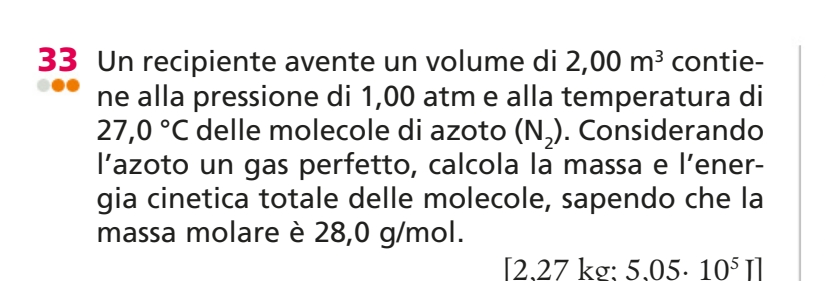
\includegraphics[width=0.85\linewidth]{immagini/es_33_traccia.png}
\caption{Traccia originale dal testo scolastico: Esercizio 33 (azoto $N_2$).}
\label{fig:es33_testo}
\end{figure}

\begin{problema}[Esercizio 33: Risoluzione Strutturata a 9 Fasi]
\begin{enumerate}[label=\textbf{Fase \arabic*:}, leftmargin=*, itemsep=5pt]
  \item \textbf{Dati del Problema:}
  \begin{itemize}[leftmargin=*, label=\textbullet]
    \item Volume del recipiente: $V = 2{,}00\,\text{m}^3$;
    \item Pressione del gas: $p = 1{,}00\,\text{atm}$;
    \item Temperatura centigrada: $t = 27{,}0\,{^\circ}\text{C}$;
    \item Sostanza: Azoto molecolare $N_2$ (molecola biatomica lineare con $l = 5$ gradi di libert\`a);
    \item Massa molare dell'azoto: $M = 28{,}0\,\text{g/mol} = 0{,}0280\,\text{kg/mol}$.
  \end{itemize}

  \item \textbf{Incognite Formalizzate:}
  \begin{itemize}[leftmargin=*, label=\textbullet]
    \item Numero di moli di gas: $n = ?\,\text{[mol]}$;
    \item Massa totale del gas confinato: $m = ?\,\text{[kg]}$;
    \item Energia cinetica totale di agitazione termica: $K_{\text{tot}} = ?\,\text{[J]}$.
  \end{itemize}

  \item \textbf{Conversione nel Sistema Internazionale (SI):}
  \begin{itemize}[leftmargin=*, label=\textbullet]
    \item $p = 1{,}00\,\text{atm} = 101325\,\text{Pa}$;
    \item $T = t + 273{,}15 = 27{,}0 + 273{,}15 = 300{,}15\,\text{K}$;
    \item $M = 0{,}0280\,\text{kg/mol}$;
    \item $V = 2{,}00\,\text{m}^3$ e $R = 8{,}314\,\text{J/(mol}\cdot\text{K)}$ (gi\`a espresse in unit\`a SI).
  \end{itemize}

  \item \textbf{Modello Fisico e Schema della Situazione:}
  Modellizziamo l'azoto come gas ideale di molecole biatomiche a manubrio rigido libere di muoversi nello spazio tridimensionale. A temperatura ambiente ($300\,\text{K}$), ciascuna molecola possiede esattamente \textbf{5 gradi di libert\`a attivi}: 3 gradi traslazionali associati alla velocit\`a del baricentro $(v_x, v_y, v_z)$ e 2 gradi rotazionali associati alla rotazione attorno ai due assi ortogonali al legame chimico $(\omega_1, \omega_2)$.
  \begin{center}
  \begin{tikzpicture}[scale=0.88, >=stealth]
    \draw[thick, slateBorder!80] (0, 0) rectangle (3.0, 2.5);
    \draw[thick, slateBorder!80] (3.0, 0) -- (4.2, 1.0) -- (4.2, 3.5) -- (3.0, 2.5);
    \draw[thick, slateBorder!80] (0, 2.5) -- (1.2, 3.5) -- (4.2, 3.5);
    \draw[dashed, slateBorder!40] (0, 0) -- (1.2, 1.0) -- (4.2, 1.0);
    \draw[dashed, slateBorder!40] (1.2, 1.0) -- (1.2, 3.5);

    \node[font=\footnotesize\bfseries, primaryBlue] at (1.8, 0.4) {$V = 2{,}00\,\text{m}^3$};
    \node[font=\scriptsize, slateBorder] at (1.8, 0.1) {$p = 1\,\text{atm},\; T = 300{,}15\,\text{K}$};

    \coordinate (O) at (1.6, 1.8);
    \draw[line width=3pt, gray!80] (1.2, 1.8) -- (2.0, 1.8);
    \fill[primaryBlue] (1.2, 1.8) circle (4pt) node[left, font=\tiny\bfseries] {$N$};
    \fill[primaryBlue] (2.0, 1.8) circle (4pt) node[right, font=\tiny\bfseries] {$N$};

    \draw[->, line width=1.5pt, accentRed] (1.6, 1.8) -- (2.6, 1.8) node[right, font=\tiny\bfseries] {$v_x$};
    \draw[->, line width=1.5pt, accentGreen!80!black] (1.6, 1.8) -- (1.6, 2.7) node[above, font=\tiny\bfseries] {$v_y$};
    \draw[->, line width=1.5pt, accentAmber] (1.6, 1.8) -- (2.2, 2.3) node[above right, font=\tiny\bfseries] {$v_z$};

    \draw[->, thick, primaryBlue] (1.6, 1.3) arc (-90:90:0.3 and 0.5) node[midway, right, font=\tiny\bfseries] {$\omega_1$};
    \draw[->, thick, primaryBlue] (2.1, 1.8) arc (0:180:0.5 and 0.25) node[midway, above, font=\tiny\bfseries] {$\omega_2$};

    \foreach \x/\y in {0.6/0.8, 0.8/2.0, 2.5/0.9, 3.3/1.7, 2.8/2.7, 1.0/1.2} {
      \fill[primaryBlue!50] (\x, \y) circle (2pt);
      \fill[primaryBlue!50] (\x+0.1, \y+0.05) circle (2pt);
      \draw[primaryBlue!80, ultra thin] (\x, \y) -- (\x+0.1, \y+0.05);
    }

    \node[draw=primaryBlue, fill=white, rounded corners=3pt, font=\scriptsize, align=left] at (6.5, 1.8) {
      \textbf{Molecola Biatomica $N_2$ ($l = 5$):}\\
      $\bullet$ $3$ gradi traslazionali ($v_x, v_y, v_z$)\\[1mm]
      $\bullet$ $2$ gradi rotazionali ($\omega_1, \omega_2$)\\[1mm]
      $\bullet$ Energia media: $\langle \epsilon \rangle = \frac{5}{2}k_B T$\\[1mm]
      $m = \dfrac{pVM}{RT} \approx \mathbf{2{,}27\,\text{kg}}$\\[1mm]
      $K_{\text{tot}} = \dfrac{5}{2}pV \approx \mathbf{5{,}05 \cdot 10^5\,\text{J}}$
    };
  \end{tikzpicture}
  \par\vspace{1.5mm}{\small\textbf{Figura 6.11:} \textit{Schema cinetico dell'Esercizio 33: la molecola biatomica di azoto $N_2$ possiede 5 gradi di libert\`a attivi a temperatura ambiente (3 traslazionali e 2 rotazionali). Per il principio di equipartizione, $K_{\text{tot}} = \frac{5}{2}pV \approx 5{,}05 \cdot 10^5\,\text{J}$.}}
  \end{center}

  \item \textbf{Leggi Fisiche Fondamentali in Forma Simbolica:}
  Dall'equazione di stato dei gas ideali:
  \[
  p V = n R T \implies n = \frac{p V}{R T}
  \]
  La massa complessiva \`e legata al numero di moli tramite la massa molare $M$:
  \[
  m = n \cdot M
  \]
  Per il Teorema di Equipartizione dell'Energia, a ciascun grado di libert\`a termicamente attivo compete un'energia cinetica media per molecola pari a $\frac{1}{2} k_B T$. Per $N_{\text{tot}} = n N_A$ molecole biatomiche con $l = 5$:
  \[
  K_{\text{tot}} = n N_A \cdot \left(\frac{5}{2} k_B T\right) = \frac{5}{2} n R T = \frac{5}{2} \, p \, V
  \]
  (la componente puramente traslazionale vale $K_{\text{trasl}} = \frac{3}{2} p V$).

  \item \textbf{Risoluzione Algebrica Simbolica Letterale:}
  Ricaviamo le formule risolutive letterali:
  \[
  \mathbf{m = \frac{p \cdot V \cdot M}{R \cdot T}} \qquad \text{e} \qquad \mathbf{K_{\text{tot}} = \frac{5}{2} \, p \, V}
  \]

  \item \textbf{Sostituzione Numerica Finale:}
  Calcoliamo il numero di moli e la massa totale:
  \[
  n = \frac{(101325\,\text{Pa}) \cdot (2{,}00\,\text{m}^3)}{(8{,}314\,\text{J/(mol}\cdot\text{K)}) \cdot (300{,}15\,\text{K})} = \frac{202650}{2495{,}45} \approx 81{,}21\,\text{mol}
  \]
  \[
  m = 81{,}21\,\text{mol} \cdot 0{,}0280\,\frac{\text{kg}}{\text{mol}} \approx \mathbf{2{,}27\,\text{kg}}
  \]
  Calcoliamo l'energia cinetica termica totale:
  \[
  K_{\text{tot}} = \frac{5}{2} \cdot (101325\,\text{Pa}) \cdot (2{,}00\,\text{m}^3) = 5 \cdot 101325\,\text{J} = 506625\,\text{J} \approx \mathbf{5{,}05 \cdot 10^5\,\text{J}}
  \]
  (di cui la sola quota traslazionale corrisponde a $K_{\text{trasl}} = \frac{3}{2} \cdot 101325 \cdot 2{,}00 \approx 3{,}04 \cdot 10^5\,\text{J}$).

  \item \textbf{Risultato Riquadrato con Unit\`a e Cifre Significative:}
  \[
  \mathbf{\boxed{m \approx 2{,}27\,\text{kg}}} \qquad \text{e} \qquad \mathbf{\boxed{K_{\text{tot}} \approx 5{,}05 \cdot 10^5\,\text{J}}}
  \]

  \item \textbf{Valutazione di Plausibilit\`a Fisica e Casi Limite:}
  \begin{itemize}[leftmargin=*, label=\textbullet]
    \item \textit{Verifica dimensionale:} $\left[\frac{p V M}{R T}\right] = \frac{\text{Pa}\cdot\text{m}^3 \cdot (\text{kg/mol})}{(\text{J}/(\text{mol}\cdot\text{K})) \cdot \text{K}} = \frac{\text{J}\cdot\text{kg/mol}}{\text{J/mol}} = \text{kg}$; $[p V] = \text{Pa}\cdot\text{m}^3 = \frac{\text{N}}{\text{m}^2}\cdot\text{m}^3 = \text{N}\cdot\text{m} = \text{J}$.
    \item \textit{Plausibilit\`a fisica:} Una densit\`a media di $\frac{2{,}27\,\text{kg}}{2{,}00\,\text{m}^3} = 1{,}14\,\text{kg/m}^3$ \`e perfettamente compatibile con la densit\`a dell'aria standard ($1{,}2\,\text{kg/m}^3$). L'energia termica cinetica microscopica supera mezzo megajoule ($0{,}51\,\text{MJ}$), rivelando l'immensa riserva energetica custodita nel moto caotico delle particelle.
    \item \textit{Casi limite:} A temperature criogeniche estremamente basse ($T \ll 100\,\text{K}$), i gradi di libert\`a rotazionali si congelano quantisticamente e il gas si comporta come monoatomico ($l \to 3 \implies K_{\text{tot}} \to \frac{3}{2}pV$); a temperature elevatissime ($T > 1000\,\text{K}$) si attivano anche i gradi vibrazionali ($l \to 7$).
  \end{itemize}
\end{enumerate}
\end{problema}


% ------------------------------------------------------------------------------
% PROBLEMA 6 (ESERCIZIO 6 DEL TESTO)
% ------------------------------------------------------------------------------
\newpage
\section{Problema 6: Confronto tra Calori Specifici — Alluminio e Ferro}

\begin{figure}[htbp]
\centering
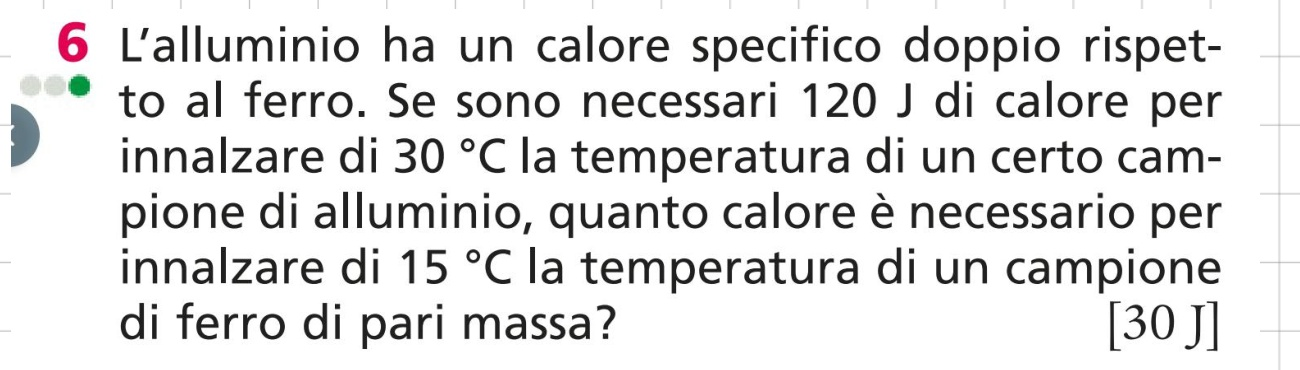
\includegraphics[width=0.85\linewidth]{immagini/es_06_traccia.jpg}
\caption{Traccia originale dal testo scolastico: Esercizio 6 (confronto calori specifici Alluminio e Ferro).}
\label{fig:es06_testo}
\end{figure}

\begin{problema}[Esercizio 6: Risoluzione Strutturata a 9 Fasi]
\begin{enumerate}[label=\textbf{Fase \arabic*:}, leftmargin=*, itemsep=5pt]
  \item \textbf{Dati del Problema:}
  \begin{itemize}[leftmargin=*, label=\textbullet]
    \item Relazione tra i calori specifici: $c_{Al} = 2 \, c_{Fe}$ (il calore specifico dell'alluminio \`e doppio rispetto a quello del ferro);
    \item Calore assorbito dal campione di alluminio: $Q_{Al} = 120\,\text{J}$;
    \item Incremento di temperatura dell'alluminio: $\Delta T_{Al} = 30\,{^\circ}\text{C} = 30\,\text{K}$;
    \item Incremento di temperatura desiderato per il ferro: $\Delta T_{Fe} = 15\,{^\circ}\text{C} = 15\,\text{K}$;
    \item Vincolo di massa: masse identiche dei due campioni ($m_{Fe} = m_{Al} = m$).
  \end{itemize}

  \item \textbf{Incognite Formalizzate:}
  \begin{itemize}[leftmargin=*, label=\textbullet]
    \item Calore necessario per innalzare la temperatura del campione di ferro: $Q_{Fe} = ?\,\text{[J]}$.
  \end{itemize}

  \item \textbf{Conversione nel Sistema Internazionale (SI):}
  \begin{itemize}[leftmargin=*, label=\textbullet]
    \item I dati sono gi\`a espressi in unit\`a coerenti del Sistema Internazionale: energia in Joule ($120\,\text{J}$);
    \item Poich\'e si tratta di differenze di temperatura, la variazione centigrada coincide esattamente con la variazione in scala assoluta: $\Delta T \, [\text{K}] = \Delta t \, [{^\circ}\text{C}]$. Dunque $\Delta T_{Al} = 30\,\text{K}$ e $\Delta T_{Fe} = 15\,\text{K}$.
  \end{itemize}

  \item \textbf{Modello Fisico e Schema della Situazione:}
  Consideriamo due campioni metallici di pari massa $m$. Il calore specifico misura la quantit\`a di energia termica necessaria per aumentare di un grado la temperatura dell'unit\`a di massa. L'alluminio ha una capacit\`a termica specifica doppia rispetto al ferro ($c_{Al} = 2 c_{Fe}$), ovvero il ferro si scalda con met\`a energia a parit\`a di massa e incremento termico. Inoltre, per il ferro \`e richiesto un salto termico dimezzato ($\Delta T_{Fe} = \frac{1}{2}\Delta T_{Al}$).
  \begin{center}
  \begin{tikzpicture}[scale=0.95, >=stealth]
    % Campione Alluminio
    \begin{scope}[shift={(0,0)}]
      \draw[very thick, primaryBlue, fill=primaryBlue!15] (0,0) rectangle (2.4, 2.2);
      \node[font=\small\bfseries, primaryBlue] at (1.2, 1.4) {Alluminio ($Al$)};
      \node[font=\footnotesize, primaryBlue] at (1.2, 1.0) {Massa $m$};
      \node[font=\footnotesize\bfseries, primaryBlue] at (1.2, 0.6) {$c_{Al} = 2\,c_{Fe}$};
      \draw[->, ultra thick, accentRed, decorate, decoration={snake, amplitude=2pt, pre length=4pt, post length=4pt}] (1.2, 3.4) -- (1.2, 2.3) node[midway, right, font=\footnotesize\bfseries, accentRed] {$Q_{Al} = 120\,\text{J}$};
      \node[draw=primaryBlue, fill=white, rounded corners=2pt, font=\scriptsize\bfseries, align=center] at (1.2, -0.6) {$\Delta T_{Al} = 30\,{^\circ}\text{C} = 30\,\text{K}$};
    \end{scope}

    \node[font=\Huge\bfseries, slateBorder!120] at (3.6, 1.1) {vs};

    % Campione Ferro
    \begin{scope}[shift={(4.8,0)}]
      \draw[very thick, slateBorder!140, fill=slateBorder!30] (0,0) rectangle (2.4, 2.2);
      \node[font=\small\bfseries, slateBorder!180] at (1.2, 1.4) {Ferro ($Fe$)};
      \node[font=\footnotesize, slateBorder!180] at (1.2, 1.0) {Massa $m$ (identica)};
      \node[font=\footnotesize\bfseries, slateBorder!180] at (1.2, 0.6) {$c_{Fe} = \frac{1}{2}\,c_{Al}$};
      \draw[->, ultra thick, accentAmber, decorate, decoration={snake, amplitude=2pt, pre length=4pt, post length=4pt}] (1.2, 3.4) -- (1.2, 2.3) node[midway, right, font=\footnotesize\bfseries, accentAmber] {$Q_{Fe} = ?$};
      \node[draw=accentGreen, fill=white, rounded corners=2pt, font=\scriptsize\bfseries, align=center] at (1.2, -0.6) {$\Delta T_{Fe} = 15\,{^\circ}\text{C} = 15\,\text{K}$\\($\frac{1}{2}$ rispetto ad $Al$)};
    \end{scope}

    % Bilancio analitico sottostante
    \node[draw=accentGreen, line width=1pt, fill=slateBg, rounded corners=3pt, font=\small\bfseries, align=center] at (3.6, -1.8) {$\displaystyle \frac{Q_{Fe}}{Q_{Al}} = \frac{c_{Fe}}{c_{Al}} \cdot \frac{\Delta T_{Fe}}{\Delta T_{Al}} = \frac{1}{2} \cdot \frac{1}{2} = \frac{1}{4} \implies \mathbf{Q_{Fe} = \frac{120\,\text{J}}{4} = 30\,\text{J}}$};
  \end{tikzpicture}
  \par\vspace{1.5mm}{\small\textbf{Figura 6.13:} \textit{Schema comparativo dell'Esercizio 6: a parit\`a di massa $m$, il campione di ferro possiede calore specifico dimezzato ($c_{Fe}/c_{Al} = 1/2$) e subisce un incremento di temperatura dimezzato ($\Delta T_{Fe}/\Delta T_{Al} = 1/2$). Il calore assorbito \`e dunque esattamente $1/4$ di quello dell'alluminio ($30\,\text{J}$).}}
  \end{center}

  \item \textbf{Leggi Fisiche Fondamentali in Forma Simbolica:}
  La legge fondamentale della calorimetria applicata ai due metalli esprime il calore scambiato in funzione della massa, del calore specifico e del gradiente termico:
  \[
  Q_{Al} = m \cdot c_{Al} \cdot \Delta T_{Al}
  \]
  \[
  Q_{Fe} = m \cdot c_{Fe} \cdot \Delta T_{Fe}
  \]

  \item \textbf{Risoluzione Algebrica Simbolica Letterale:}
  Dividendo membro a membro la seconda equazione per la prima, la massa incognita $m$ si elide perfettamente:
  \[
  \frac{Q_{Fe}}{Q_{Al}} = \frac{m \cdot c_{Fe} \cdot \Delta T_{Fe}}{m \cdot c_{Al} \cdot \Delta T_{Al}} = \left(\frac{c_{Fe}}{c_{Al}}\right) \cdot \left(\frac{\Delta T_{Fe}}{\Delta T_{Al}}\right)
  \]
  Sostituendo la relazione $c_{Al} = 2 c_{Fe} \iff \frac{c_{Fe}}{c_{Al}} = \frac{1}{2}$:
  \[
  \mathbf{Q_{Fe} = Q_{Al} \cdot \frac{1}{2} \cdot \frac{\Delta T_{Fe}}{\Delta T_{Al}}}
  \]

  \item \textbf{Sostituzione Numerica Finale:}
  Inserendo i valori numerici assegnati dal problema:
  \[
  Q_{Fe} = 120\,\text{J} \cdot \frac{1}{2} \cdot \frac{15\,\text{K}}{30\,\text{K}} = 120\,\text{J} \cdot \frac{1}{2} \cdot \frac{1}{2} = \frac{120\,\text{J}}{4} = \mathbf{30\,\text{J}}
  \]

  \item \textbf{Risultato Riquadrato con Unit\`a e Cifre Significative:}
  \[
  \mathbf{\boxed{Q_{Fe} = 30\,\text{J}}}
  \]

  \item \textbf{Valutazione di Plausibilit\`a Fisica e Casi Limite:}
  \begin{itemize}[leftmargin=*, label=\textbullet]
    \item \textit{Verifica dimensionale:} $\left[Q_{Al} \cdot \frac{c_{Fe}}{c_{Al}} \cdot \frac{\Delta T_{Fe}}{\Delta T_{Al}}\right] = \text{J} \cdot 1 \cdot 1 = \text{J}$, dimensionalmente coerente.
    \item \textit{Plausibilit\`a fisica:} Il calore specifico misura l'energia per scaldare l'unit\`a di massa. Avendo il ferro un'inerzia termica dimezzata e dovendo compiere un salto termico dimezzato, l'energia richiesta crolla di un fattore $2 \times 2 = 4$. Il risultato numerico $30\,\text{J}$ coincide esattamente con la soluzione ufficiale del libro.
    \item \textit{Casi limite:} Se $\Delta T_{Fe} \to 0$, $Q_{Fe} \to 0$; se $c_{Fe} \to c_{Al}$ e $\Delta T_{Fe} \to \Delta T_{Al}$, $Q_{Fe} \to Q_{Al} = 120\,\text{J}$.
  \end{itemize}
\end{enumerate}
\end{problema}

% ------------------------------------------------------------------------------
% PROBLEMA 7 (ESERCIZIO 8 DEL TESTO)
% ------------------------------------------------------------------------------
\newpage
\section{Problema 7: Energia Termica in un Ciclo di Lavatrice e Calcolo in Kilowattora}

\begin{figure}[htbp]
\centering
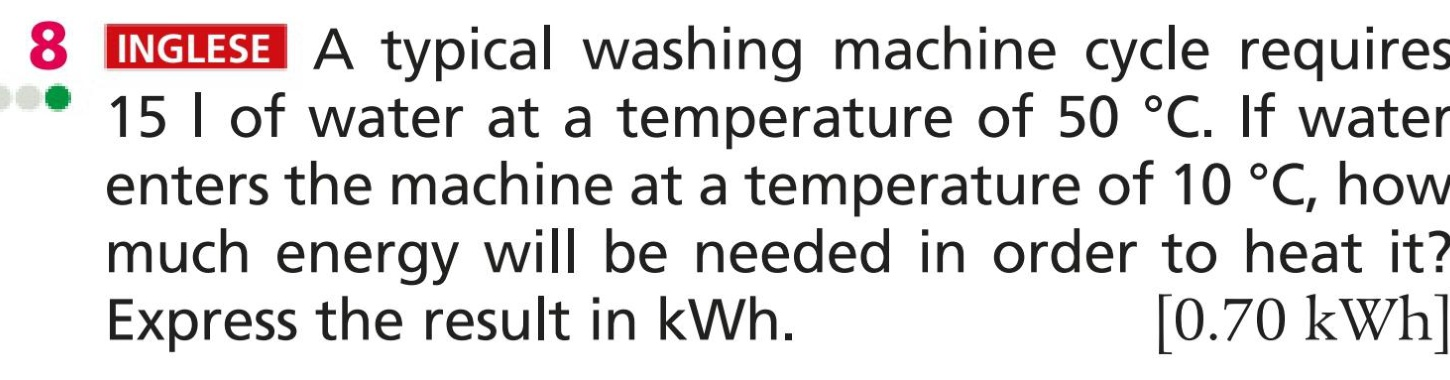
\includegraphics[width=0.85\linewidth]{immagini/es_08_traccia.jpg}
\caption{Traccia originale dal testo scolastico: Esercizio 8 (energia riscaldamento acqua lavatrice in kWh).}
\label{fig:es08_testo}
\end{figure}

\begin{problema}[Esercizio 8: Risoluzione Strutturata a 9 Fasi]
\begin{enumerate}[label=\textbf{Fase \arabic*:}, leftmargin=*, itemsep=5pt]
  \item \textbf{Dati del Problema:}
  \begin{itemize}[leftmargin=*, label=\textbullet]
    \item Volume d'acqua utilizzato dalla lavatrice nel ciclo: $V = 15\,\text{L}$;
    \item Temperatura finale di lavaggio: $T_f = 50\,{^\circ}\text{C}$;
    \item Temperatura iniziale dell'acqua di rete in ingresso: $T_i = 10\,{^\circ}\text{C}$;
    \item Densit\`a volumica dell'acqua: $\rho_{\text{acqua}} = 1{,}00 \cdot 10^3\,\text{kg/m}^3 = 1{,}00\,\text{kg/L}$;
    \item Calore specifico dell'acqua liquida: $c_{\text{acqua}} = 4186\,\text{J/(kg}\cdot\text{K)}$;
    \item Fattore di conversione Joule-Kilowattora: $1\,\text{kWh} = 3{,}60 \cdot 10^6\,\text{J}$.
  \end{itemize}

  \item \textbf{Incognite Formalizzate:}
  \begin{itemize}[leftmargin=*, label=\textbullet]
    \item Massa d'acqua complessiva da riscaldare: $m = ?\,\text{[kg]}$;
    \item Energia termica assorbita dall'acqua espressa in Joule: $Q = ?\,\text{[J]}$;
    \item Energia termica espressa in kilowattora: $E = ?\,\text{[kWh]}$.
  \end{itemize}

  \item \textbf{Conversione nel Sistema Internazionale (SI):}
  \begin{itemize}[leftmargin=*, label=\textbullet]
    \item $V = 15\,\text{L} = 15 \cdot 10^{-3}\,\text{m}^3 \implies m = \rho \cdot V = 1{,}00\,\text{kg/L} \cdot 15\,\text{L} = 15{,}0\,\text{kg}$;
    \item $\Delta T = T_f - T_i = 50\,{^\circ}\text{C} - 10\,{^\circ}\text{C} = 40\,{^\circ}\text{C} = 40\,\text{K}$;
    \item $c = 4186\,\text{J/(kg}\cdot\text{K)}$.
  \end{itemize}

  \item \textbf{Modello Fisico e Schema della Situazione:}
  L'acqua entra nel cestello della lavatrice a temperatura ambiente ($10^\circ\text{C}$). Una resistenza elettrica corazzata immersa nel liquido dissipa potenza elettrica per effetto Joule ($P = R I^2$), trasformando energia potenziale elettrica in flusso termico continuo assorbito dalla massa d'acqua fino a raggiungere i $50^\circ\text{C}$ programmati. Un contatore elettrico a monte registra il prelievo energetico dalla rete in $\text{kWh}$.
  \begin{center}
  \begin{tikzpicture}[scale=0.92, >=stealth]
    % Corpo lavatrice
    \draw[very thick, primaryBlue, fill=slateBg, rounded corners=4pt] (0,0) rectangle (4.2, 4.0);
    % Oblò circolare
    \draw[line width=2pt, slateBorder!120, fill=white] (2.1, 2.0) circle (1.4);
    \fill[primaryBlue!20] (0.85, 1.6) arc (195:345:1.3) -- (3.35, 1.6) -- cycle;
    \draw[thick, primaryBlue] (0.85, 1.6) -- (3.35, 1.6) node[midway, above, font=\scriptsize\bfseries, primaryBlue] {Acqua: $V = 15\,\text{L} \implies m = 15\,\text{kg}$};
    \node[font=\tiny\bfseries, primaryBlue] at (2.1, 1.1) {$T_i = 10\,{^\circ}\text{C} \xrightarrow{\Delta T = 40\,\text{K}} T_f = 50\,{^\circ}\text{C}$};

    % Resistenza elettrica scaldante
    \draw[line width=2pt, accentRed, decorate, decoration={coil, aspect=0.7, segment length=4mm, amplitude=3mm}] (1.2, 0.6) -- (3.0, 0.6);
    \node[below, font=\tiny\bfseries, accentRed] at (2.1, 0.3) {Resistenza scaldante (Effetto Joule)};

    % Display comandi lavatrice
    \draw[thick, fill=slateBorder!40] (0.4, 3.4) rectangle (3.8, 3.8);
    \node[font=\scriptsize\bfseries, primaryBlue] at (2.1, 3.6) {LAVAGGIO $50\,{^\circ}\text{C}$ -- CICLO ECO};

    % Flusso energia e contatore kWh
    \draw[->, ultra thick, accentAmber] (5.2, 2.0) -- (4.3, 2.0) node[midway, above, font=\scriptsize\bfseries, align=center] {Energia\\Elettrica};
    
    \begin{scope}[shift={(5.4, 0.8)}]
      \draw[thick, primaryBlue, fill=white, rounded corners=3pt] (0,0) rectangle (2.8, 2.4);
      \node[font=\footnotesize\bfseries, primaryBlue] at (1.4, 2.1) {Contatore kWh};
      \draw[fill=black] (0.3, 1.1) rectangle (2.5, 1.7);
      \node[font=\small\bfseries\ttfamily, accentGreen] at (1.4, 1.4) {0000.70 kWh};
      \node[font=\scriptsize, align=center] at (1.4, 0.6) {$Q = 2{,}51 \cdot 10^6\,\text{J}$\\$E \approx 0{,}70\,\text{kWh}$};
    \end{scope}
  \end{tikzpicture}
  \par\vspace{1.5mm}{\small\textbf{Figura 6.14:} \textit{Schema termomeccanico dell'Esercizio 8: la resistenza elettrica a immersione riscalda $15\,\text{L}$ di acqua liquida producendo un salto termico $\Delta T = 40\,\text{K}$. L'energia assorbita \`e pari a $2{,}51 \cdot 10^6\,\text{J}$, equivalente a circa $0{,}70\,\text{kWh}$ registrati dal contatore elettrico.}}
  \end{center}

  \item \textbf{Leggi Fisiche Fondamentali in Forma Simbolica:}
  La massa d'acqua \`e legata al volume mediante la densit\`a:
  \[
  m = \rho_{\text{acqua}} \cdot V
  \]
  La legge fondamentale della calorimetria determina il calore in Joule:
  \[
  Q = m \cdot c \cdot \Delta T = \rho_{\text{acqua}} \cdot V \cdot c_{\text{acqua}} \cdot (T_f - T_i)
  \]
  La conversione in kilowattora avviene dividendo per il fattore di equivalenza $3{,}60 \cdot 10^6\,\text{J/kWh}$:
  \[
  E_{[\text{kWh}]} = \frac{Q_{[\text{J}]}}{3{,}60 \cdot 10^6\,\text{J/kWh}}
  \]

  \item \textbf{Risoluzione Algebrica Simbolica Letterale:}
  Sostituendo direttamente la formulazione calorimetrica nella relazione di conversione:
  \[
  \mathbf{E = \frac{\rho \cdot V \cdot c \cdot (T_f - T_i)}{3{,}60 \cdot 10^6}}
  \]

  \item \textbf{Sostituzione Numerica Finale:}
  Calcoliamo anzitutto il calore assorbito in Joule:
  \[
  Q = 15{,}0\,\text{kg} \cdot 4186\,\frac{\text{J}}{\text{kg}\cdot\text{K}} \cdot 40\,\text{K} = 2\,511\,600\,\text{J} \approx \mathbf{2{,}51 \cdot 10^6\,\text{J}}
  \]
  Convertiamo in kilowattora:
  \[
  E = \frac{2\,511\,600\,\text{J}}{3{,}60 \cdot 10^6\,\text{J/kWh}} \approx 0{,}69766...\,\text{kWh} \approx \mathbf{0{,}70\,\text{kWh}}
  \]

  \item \textbf{Risultato Riquadrato con Unit\`a e Cifre Significative:}
  \[
  \mathbf{\boxed{Q \approx 2{,}51 \cdot 10^6\,\text{J} = 2{,}51\,\text{MJ}}} \qquad \text{e} \qquad \mathbf{\boxed{E \approx 0{,}70\,\text{kWh}}}
  \]

  \item \textbf{Valutazione di Plausibilit\`a Fisica e Casi Limite:}
  \begin{itemize}[leftmargin=*, label=\textbullet]
    \item \textit{Verifica dimensionale:} $\left[\frac{\text{kg} \cdot (\text{J/(kg}\cdot\text{K)}) \cdot \text{K}}{\text{J/kWh}}\right] = \frac{\text{J}}{\text{J/kWh}} = \text{kWh}$, impeccabile.
    \item \textit{Plausibilit\`a fisica e consumo reale:} Una lavatrice moderna in classe di efficienza media consuma circa $0{,}7\text{--}1{,}0\,\text{kWh}$ a ciclo per il riscaldamento a $50^\circ\text{C}$. Con una tariffa media di $0{,}25\,\text{EUR/kWh}$, il costo della sola energia termica per un lavaggio ammonta a circa $0{,}70 \times 0{,}25 \approx 0{,}18\,\text{EUR}$.
    \item \textit{Casi limite:} Se $T_f = T_i$ (lavaggio a freddo), $\Delta T = 0 \implies E = 0\,\text{kWh}$; l'energia necessaria cresce in modo strettamente lineare con la temperatura impostata.
  \end{itemize}
\end{enumerate}
\end{problema}

% ------------------------------------------------------------------------------
% PROBLEMA 8 (ESERCIZIO 10 DEL TESTO)
% ------------------------------------------------------------------------------
\newpage
\section{Problema 8: Lavoro Muscolare su una Scala e Dissipazione Termica Umana}

\begin{figure}[htbp]
\centering
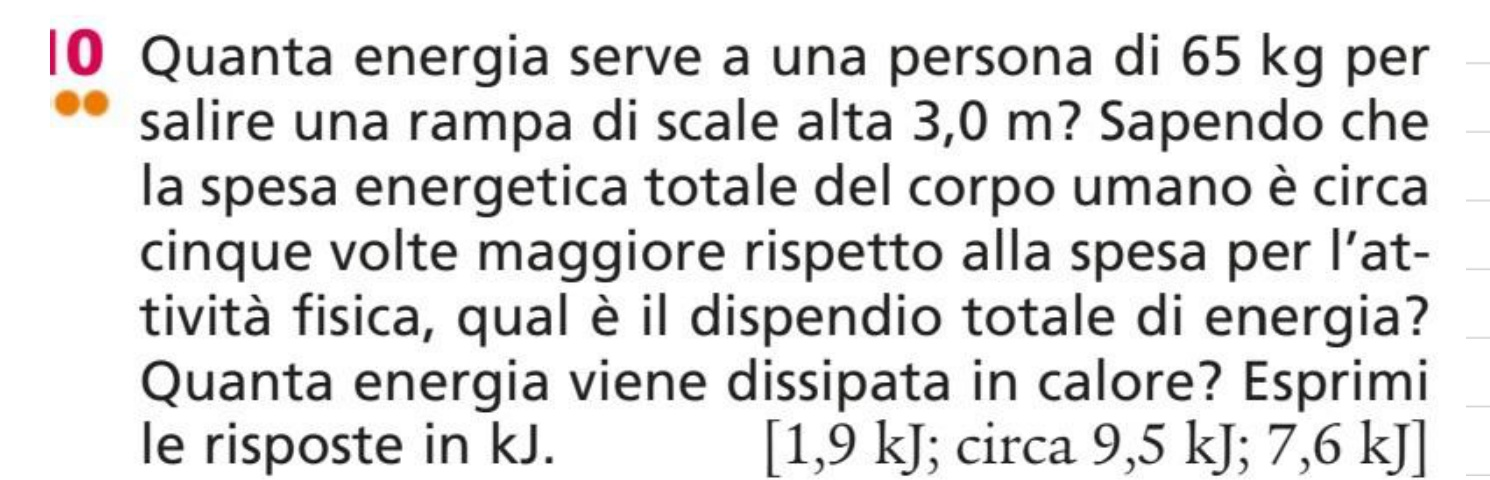
\includegraphics[width=0.85\linewidth]{immagini/es_10_traccia.jpg}
\caption{Traccia originale dal testo scolastico: Esercizio 10 (dispendio energetico e calore dissipato).}
\label{fig:es10_testo}
\end{figure}

\begin{problema}[Esercizio 10: Risoluzione Strutturata a 9 Fasi]
\begin{enumerate}[label=\textbf{Fase \arabic*:}, leftmargin=*, itemsep=5pt]
  \item \textbf{Dati del Problema:}
  \begin{itemize}[leftmargin=*, label=\textbullet]
    \item Massa della persona: $m = 65\,\text{kg}$;
    \item Dislivello verticale superato: $h = 3{,}0\,\text{m}$;
    \item Accelerazione gravitazionale standard: $g = 9{,}81\,\text{m/s}^2$;
    \item Fattore di spesa metabolica totale del corpo umano rispetto al lavoro meccanico utile: $k = 5$ ($E_{\text{tot}} \approx 5 \cdot L_{\text{mecc}}$);
    \item Rendimento muscolare implicito: $\eta = \frac{L}{E_{\text{tot}}} = \frac{1}{5} = 0{,}20 = 20\%$.
  \end{itemize}

  \item \textbf{Incognite Formalizzate:}
  \begin{itemize}[leftmargin=*, label=\textbullet]
    \item Lavoro meccanico utile contro la gravit\`a per salire la scala: $L = ?\,\text{[kJ]}$;
    \item Dispendio energetico metabolico totale consumato dall'organismo: $E_{\text{tot}} = ?\,\text{[kJ]}$;
    \item Quantit\`a di energia biochimica dissipata sotto forma di calore: $Q = ?\,\text{[kJ]}$.
  \end{itemize}

  \item \textbf{Conversione nel Sistema Internazionale (SI):}
  \begin{itemize}[leftmargin=*, label=\textbullet]
    \item Le grandezze sono fornite direttamente in unit\`a coerenti: massa $65\,\text{kg}$, quota $3{,}0\,\text{m}$, accelerazione $9{,}81\,\text{m/s}^2$;
    \item I risultati finali devono essere convertiti in chilojoule ($\text{kJ}$), ricordando che $1\,\text{kJ} = 10^3\,\text{J}$.
  \end{itemize}

  \item \textbf{Modello Fisico e Schema della Situazione:}
  Salendo una scala a velocit\`a di regime costante, le forze muscolari compiono un lavoro positivo contro la forza peso $\vec{P} = m\vec{g}$. Per il Primo Principio della Termodinamica applicato alla macchina termochimica umana, l'energia metabolica interna liberata dall'idrolisi dell'ATP ($E_{\text{tot}}$) non pu\`o essere trasformata integralmente in lavoro utile per i vincoli dell'efficienza muscolare ($\eta \approx 20\%$); la restante frazione ($80\%$) viene convertita in calore interno $Q$, che innalza la temperatura corporea e deve essere espulso tramite convezione e sudorazione.
  \begin{center}
  \begin{tikzpicture}[scale=0.92, >=stealth]
    % Rampa di scale
    \draw[very thick, slateBorder!140, fill=slateBorder!20] 
      (0,0) -- (1.0,0) -- (1.0,0.8) -- (2.0,0.8) -- (2.0,1.6) -- (3.0,1.6) -- (3.0,2.4) -- (4.0,2.4) -- (4.0,3.2) -- (4.0,0) -- cycle;
    % Quota verticale h
    \draw[<->, thick, primaryBlue] (4.4, 0) -- (4.4, 3.2) node[midway, right, font=\footnotesize\bfseries] {$h = 3{,}0\,\text{m}$};

    % Persona stilizzata sullo scalino
    \begin{scope}[shift={(2.5, 2.4)}]
      \draw[thick, primaryBlue] (0, 0) circle (0.2);
      \draw[thick, primaryBlue] (0, -0.2) -- (0, -0.8);
      \draw[thick, primaryBlue] (0, -0.4) -- (-0.3, -0.6);
      \draw[thick, primaryBlue] (0, -0.4) -- (0.3, -0.6);
      \draw[thick, primaryBlue] (0, -0.8) -- (-0.2, -1.3);
      \draw[thick, primaryBlue] (0, -0.8) -- (0.2, -1.3);
      \node[above, font=\scriptsize\bfseries, primaryBlue] at (0, 0.25) {$m = 65\,\text{kg}$};
      % Vettore peso
      \draw[->, line width=1.5pt, accentRed] (0, -0.5) -- (0, -1.5) node[right, font=\scriptsize\bfseries] {$\vec{P} = m\vec{g}$};
      % Vettore forza muscolare
      \draw[->, line width=1.5pt, accentGreen] (0, -0.5) -- (0, 0.5) node[left, font=\scriptsize\bfseries] {$\vec{F}_{\text{musc}}$};
    \end{scope}

    % Diagramma a barre dell'energia
    \begin{scope}[shift={(5.8, 0.2)}]
      \draw[thick, slateBorder] (-0.2, 0) -- (3.4, 0);
      % Spesa totale (100%)
      \fill[primaryBlue!30] (0, 0) rectangle (0.8, 3.0);
      \draw[thick, primaryBlue] (0, 0) rectangle (0.8, 3.0);
      \node[above, font=\scriptsize\bfseries, primaryBlue] at (0.4, 3.0) {$E_{\text{tot}} \approx 9{,}5\,\text{kJ}$};
      \node[font=\tiny\bfseries, primaryBlue, align=center] at (0.4, 1.5) {Spesa\\Metabolica\\$100\%$};

      % Lavoro utile (20%)
      \fill[accentGreen!35] (1.2, 0) rectangle (2.0, 0.6);
      \draw[thick, accentGreen] (1.2, 0) rectangle (2.0, 0.6);
      \node[above, font=\scriptsize\bfseries, accentGreen] at (1.6, 0.6) {$L \approx 1{,}9\,\text{kJ}$};
      \node[font=\tiny\bfseries, accentGreen] at (1.6, 0.3) {$20\%$ Utile};

      % Calore dissipato (80%)
      \fill[accentAmber!35] (2.2, 0) rectangle (3.0, 2.4);
      \draw[thick, accentAmber] (2.2, 0) rectangle (3.0, 2.4);
      \node[above, font=\scriptsize\bfseries, accentAmber] at (2.6, 2.4) {$Q \approx 7{,}6\,\text{kJ}$};
      \node[font=\tiny\bfseries, accentAmber, align=center] at (2.6, 1.2) {$80\%$\\Dissipato\\in Calore};
    \end{scope}
  \end{tikzpicture}
  \par\vspace{1.5mm}{\small\textbf{Figura 6.15:} \textit{Bilancio biomeccanico dell'Esercizio 10: per salire il dislivello $h = 3{,}0\,\text{m}$, la persona compie un lavoro meccanico contro la gravit\`a pari a $L = mgh \approx 1{,}9\,\text{kJ}$. Poich\'e il rendimento muscolare \`e del $20\%$ ($k = 5$), l'organismo consuma $E_{\text{tot}} \approx 9{,}5\,\text{kJ}$ e dissipa ben $7{,}6\,\text{kJ}$ sotto forma di calore corporeo.}}
  \end{center}

  \item \textbf{Leggi Fisiche Fondamentali in Forma Simbolica:}
  Il lavoro meccanico compiuto contro la forza gravitazionale corrisponde alla variazione di energia potenziale gravitazionale:
  \[
  L = \Delta U_g = m \cdot g \cdot h
  \]
  La spesa energetica metabolica complessiva \`e proporzionale al lavoro secondo il fattore biologico $k = 5$:
  \[
  E_{\text{tot}} = 5 \cdot L = 5 \, m \, g \, h
  \]
  Il bilancio energetico di conservazione sancisce che la quota non convertita in lavoro meccanico viene interamente dispersa in calore:
  \[
  E_{\text{tot}} = L + Q \implies Q = E_{\text{tot}} - L = 4 \cdot L = 4 \, m \, g \, h
  \]

  \item \textbf{Risoluzione Algebrica Simbolica Letterale:}
  Formuliamo le tre incognite in termini delle grandezze fondamentali del problema:
  \[
  \mathbf{L = m \cdot g \cdot h}
  \]
  \[
  \mathbf{E_{\text{tot}} = 5 \, m \, g \, h}
  \]
  \[
  \mathbf{Q = 4 \, m \, g \, h}
  \]

  \item \textbf{Sostituzione Numerica Finale:}
  Calcoliamo il lavoro meccanico utile:
  \[
  L = 65\,\text{kg} \cdot 9{,}81\,\frac{\text{m}}{\text{s}^2} \cdot 3{,}0\,\text{m} = 1912{,}95\,\text{J} \approx \mathbf{1{,}91\,\text{kJ}} \approx \mathbf{1{,}9\,\text{kJ}}
  \]
  Calcoliamo il dispendio energetico totale:
  \[
  E_{\text{tot}} = 5 \cdot 1912{,}95\,\text{J} = 9564{,}75\,\text{J} \approx \mathbf{9{,}56\,\text{kJ}} \approx \mathbf{9{,}5\,\text{kJ}}
  \]
  Calcoliamo l'energia dissipata in calore:
  \[
  Q = 9564{,}75\,\text{J} - 1912{,}95\,\text{J} = 7651{,}8\,\text{J} \approx \mathbf{7{,}65\,\text{kJ}} \approx \mathbf{7{,}6\,\text{kJ}}
  \]

  \item \textbf{Risultato Riquadrato con Unit\`a e Cifre Significative:}
  \[
  \mathbf{\boxed{L \approx 1{,}9\,\text{kJ}}} \qquad \mathbf{\boxed{E_{\text{tot}} \approx 9{,}5\,\text{kJ}}} \qquad \mathbf{\boxed{Q \approx 7{,}6\,\text{kJ}}}
  \]

  \item \textbf{Valutazione di Plausibilit\`a Fisica e Casi Limite:}
  \begin{itemize}[leftmargin=*, label=\textbullet]
    \item \textit{Verifica dimensionale:} $[mgh] = \text{kg} \cdot (\text{m/s}^2) \cdot \text{m} = \text{N} \cdot \text{m} = \text{J} = 10^{-3}\,\text{kJ}$, perfetta.
    \item \textit{Plausibilit\`a fisiologica:} I muscoli scheletrici possiedono un rendimento biologico reale dell'ordine del $20\text{--}25\%$. Ben l'$80\%$ dell'energia consumata dall'idrolisi degli zuccheri e dei grassi si tramuta inevitabilmente in calore, spiegando perch\'e un'intensa attivit\`a fisica determini una rapida sudorazione necessaria per mantenere l'omeostasi termica a $37\,{^\circ}\text{C}$.
    \item \textit{Casi limite:} Per un dislivello nullo ($h = 0$) il lavoro gravitazionale netto si annulla ($L = 0$); in una macchina ideale reversibile con rendimento unitario ($100\%$, $k = 1$), non vi sarebbe alcuna dispersione termica ($Q = 0$).
  \end{itemize}
\end{enumerate}
\end{problema}

\end{document}
